\documentclass{book}

\usepackage{fancyhdr}
\usepackage[utf8]{inputenc}
\usepackage[spanish,es-nodecimaldot]{babel}

\usepackage{dsfont}

\usepackage{ifxetex}
\usepackage{ifpdf}

\usepackage{xargs}
\usepackage[pdftex,dvipsnames]{xcolor}
\usepackage[colorinlistoftodos,prependcaption,textsize=tiny]{todonotes}
\newcommandx{\unsure}[2][1=]{\todo[linecolor=red,backgroundcolor=red!25,bordercolor=red,#1]{#2}}
\newcommandx{\change}[2][1=]{\todo[linecolor=blue,backgroundcolor=blue!25,bordercolor=blue,#1]{#2}}
\newcommandx{\info}[2][1=]{\todo[linecolor=OliveGreen,backgroundcolor=OliveGreen!25,bordercolor=OliveGreen,#1]{#2}}
\newcommandx{\improvement}[2][1=]{\todo[linecolor=Plum,backgroundcolor=Plum!25,bordercolor=Plum,#1]{#2}}
\newcommandx{\thiswillnotshow}[2][1=]{\todo[disable,#1]{#2}}


\vsize=27.9cm \hsize=21cm \setlength{\textwidth}{16cm}
\setlength{\textheight}{21.5cm}
\setlength{\oddsidemargin}{0.0cm}
\setlength{\evensidemargin}{0.0cm}
%\setlength{\topmargin}{-1.5cm}
\parskip 5pt

%%%%%%%%%%%%% Packages %%%%%%%%%%%%%%%%%
\usepackage{amssymb, amsthm,amsmath}
\usepackage{bm}

\ifpdf
  \usepackage{graphicx}
  \usepackage{hyperref}
\else
  \ifxetex
    \usepackage{graphicx}
    \usepackage{hyperref}
  \else
    \usepackage[dvipdfm]{graphicx}
    \usepackage[dvipdfm]{hyperref}
  \fi
\fi

\graphicspath{ {../imagenes/} }

\usepackage{enumitem}
\setenumerate[0]{label=(\alph*)}

\usepackage{caption}
\usepackage{soul, color}

\usepackage{listings}
\lstset{
  frame=single,
  breaklines=true,
  basicstyle=\fontsize{7}{13}\selectfont\ttfamily
}

%%%%%%%%%%%% algo and keywords %%%%%%%
\usepackage[ruled]{algorithm2e}
\SetKw{KwGoto}{goto}
\SetKwRepeat{OnError}{try}{on error}
%%%%%%%%%%%% hyperref %%%%%%%
\hypersetup{
bookmarksnumbered=true,
colorlinks=true,
pdfstartview={FitH},
linkcolor=blue
}

%%%%%%%%%%%%%%%%%%%%%%%%%%%%%%%%%%%%%%%
\newcommand\sep{\,:\,}
\newcommand{\vSpace}{\vspace{5mm}\noindent}
\newcommand{\vSmall}{\vspace{3mm}\noindent}
\newcommand\fakesection[1]{\noindent{\bf #1}\\}
\newcommand\bs{\backslash}

\usepackage{listings}
\lstset{
  basicstyle=\ttfamily,
  columns=fullflexible,
}

\usepackage{url}
\usepackage{multicol}
\usepackage{dsfont}

% Bold symbols for vectors and matrices
\newcommand{\xstar}{\bm{x}^{\star}}
\newcommand{\alphab}{\bm{\alpha}}
\newcommand{\ab}{\bm{a}}
\newcommand{\bb}{\bm{b}}
\newcommand{\cb}{\bm{c}}
\newcommand{\db}{\bm{d}}
\newcommand{\eb}{\bm{e}}
\newcommand{\gb}{\bm{g}}
\newcommand{\mb}{\bm{m}}
\newcommand{\pb}{\bm{p}}
\newcommand{\qb}{\bm{q}}
\newcommand{\rb}{\bm{r}}
\newcommand{\ssb}{\bm{s}}
\newcommand{\ub}{\bm{u}}
\newcommand{\vb}{\bm{v}}
\newcommand{\wb}{\bm{w}}
\newcommand{\xb}{\bm{x}}
\newcommand{\yb}{\bm{y}}
\newcommand{\zb}{\bm{z}}

\newcommand{\Ab}{\bm{A}}
\newcommand{\Bb}{\bm{B}}
\newcommand{\Cb}{\bm{C}}
\newcommand{\Db}{\bm{D}}
\newcommand{\Eb}{\bm{E}}
\newcommand{\Fb}{\bm{F}}
\newcommand{\Gb}{\bm{G}}
\newcommand{\Hb}{\bm{H}}
\newcommand{\Ib}{\bm{I}}
\newcommand{\Id}{\bm{I}}
\newcommand{\Kb}{\bm{K}}
\newcommand{\Lb}{\bm{L}}
\newcommand{\Mb}{\bm{M}}
\newcommand{\Pb}{\bm{P}}
\newcommand{\Qb}{\bm{Q}}
\newcommand{\Rb}{\bm{R}}
\newcommand{\Sb}{\bm{S}}
\newcommand{\Tb}{\bm{T}}
\newcommand{\Ub}{\bm{U}}
\newcommand{\Vb}{\bm{V}}
\newcommand{\Wb}{\bm{W}}
\newcommand{\Xb}{\bm{X}}
\newcommand{\Yb}{\bm{Y}}
\newcommand{\Zb}{\bm{Z}}
\newcommand{\Lambdab}{\bm{\Lambda}}
\newcommand{\cero}{\bm{0}}

% Rings and fields
\newcommand{\A}{\mathbb{A}}
\newcommand{\Z}{\mathbb{Z}}
\newcommand{\Q}{\mathbb{Q}}
\newcommand{\C}{\mathbb{C}}
\newcommand{\R}{\mathbb{R}}
\newcommand{\K}{\mathbb{K}}
\newcommand{\N}{\mathbb{N}}

\newcommand{\borel}{{\mathcal B}}
\newcommand{\pmom}{{\rho_{\text{mom}}}}
\newcommand{\MX}{{\mathcal{M}(X)}}


% Inner product
\newcommand{\innerl}[2]{\langle #1, #2 \rangle}
\newcommand{\inner}[2]{#1 \boldsymbol{\cdot} #2}
\newcommand{\innerTrace}[2]{#1 \bullet #2}

% Symmetric and positive definite matrices
\newcommand{\Splusplusn}{{\mathcal S_{++}^n}}
\newcommand{\Splusn}{{\mathcal S_+^n}}
\newcommand{\Splus}{{\mathcal S_+}}
\newcommand{\Sym}{{\mathcal S}}
\newcommand{\Symn}{{\mathcal S^n}}

% Cones
\newcommand\CC{\mathcal{C}}
\DeclareMathOperator{\cone}{cono}
\DeclareMathOperator{\conv}{conv}
\DeclareMathOperator{\supp}{supp}


% Spectrahedron
\newcommand{\eLL}{{\mathcal L}}

% Matrices and vectors over R or C
\newcommand{\Rnn}{\R^{n\times n}}
\newcommand{\Cnn}{\C^{n\times n}}
\newcommand{\Rn}{\R^{n}}
\newcommand{\Rm}{\R^{m}}


% Math operators
\DeclareMathOperator{\Tr}{Tr}
\DeclareMathOperator{\tr}{Tr}
\DeclareMathOperator{\interior}{int}
\DeclareMathOperator{\rank}{rank}
\DeclareMathOperator{\diag}{diag}

\newcommand\one{\mathds{1}} 

%\newcommand\one{\mathds{1}}
\newcommand\kk{\Bbbk}

\newcommand\algno{\overline\Q}

\newcommand\wo[1]{\backslash{\{#1\}}}
\newcommand\spn[1]{\langle #1 \rangle}
\newcommand{\ux}{\underline x}
\newcommand\authortext[1]{\ifforauthor {\color{red}#1} \fi}
\renewcommand\st{\mathrel{\ooalign{$\,\backepsilon$\cr\lower .7pt\hbox{\kern 1pt$-\,$}}}}
\newcommand\bref[3][blue]{%
  \begingroup%
  \hypersetup{linkcolor=#1}%
  \hyperlink{#2}{#3}%
  \endgroup}




%%%%%%%%%%%%%%% TITLE %%%%%%%%
%\title{Template for TeX files}
\title{}
\date{}
\thispagestyle{empty}
%%%%%%%%%%%%%%%%%%%%%%%%%%%
\theoremstyle{plain}
\newtheorem{theorem}{Teorema}[chapter]
\newtheorem{definition}[theorem]{Definición}
\newtheorem{conjecture}[theorem]{Conjectura}
\newtheorem{lemma}[theorem]{Lema}
\newtheorem{coro}[theorem]{Corolario}
\newtheorem{corollary}[theorem]{Corolario}
\newtheorem{proposition}[theorem]{Proposición}
\newtheorem{prop}[theorem]{Proposición}

\theoremstyle{definition}
\newtheorem{exercise}[theorem]{Ejercicio}
\newtheorem{ejercicio}[theorem]{Ejercicio}
\newtheorem{problem}[theorem]{Problema}
\newtheorem{example}[theorem]{Ejemplo}
\newtheorem{remark}[theorem]{Observación}
\newtheorem*{notation}{Notación}


%%% free theorem styles
\newcommand{\thistheoremname}{}
\newtheorem{genericthm}[theorem]{\thistheoremname}
\newenvironment{namedthm}[1]
  {\renewcommand{\thistheoremname}{#1}%
   \begin{genericthm}}
  {\end{genericthm}}
\newtheorem{none}[theorem]{}


\title{Optimizaci\'on semidefinida}

\author{Santiago Laplagne}
%\address{Instituto de C\'alculo, FCEN, Universidad de Buenos Aires - Ciudad Universitaria,
%Pabell\'on I - (C1428EGA) - Buenos Aires, Argentina}
%\email{slaplagn@dm.uba.ar}

\begin{document}

\maketitle

\tableofcontents

%\include{chapterPreliminares}

%\pagebreak

\chapter*{Prefacio}
Estas notas fueron elaboradas para el curso de Optimización Semidefinida dictado en el Segundo Cuatrimestre de 2021 en la Facultad de Ciencias Exactas y Naturales de la Universidad de Buenos Aires. La mayor parte del material en estas notas es traducción de otros textos, que se referencian al principio de la sección correspondiente. No hay ninguna intención de originalidad en estas notas sino que se presentan como una recopilación y traducción de material para facilitar la cursada a los alumnos y alumnas del curso.

\chapter{Programaci\'on lineal}

\section{Introducci\'on}

Programaci\'on lineal es el problema de minimizar o maximizar una funci\'on lineal sujeta a restricciones lineales.

Comenzamos con un ejemplo simple (\cite[Capítulo 9.3]{Cengage}. Queremos maximizar la función
$$f(x_1, x_2) = 4x_1 + 6x_2$$
sujeta a las restricciones
\begin{alignat*}{2}
   & \quad & -x_1 + x_2 &\le 11 \\
   &   \quad & x_1 + x_2 &\le 27 \\
   &   \quad & 2x_1 + 5x_2 &\le 90 \\
   & &  x_1, x_2 &\ge 0.
\end{alignat*}

Cada una de las desigualdades en las restricciones define un semiplano en $\R^2$.
Podemos graficar el conjunto de todos los puntos de $\R^2$ que cumplen todas las restricciones intersecando los semiplanos correspondientes.

\begin{center}
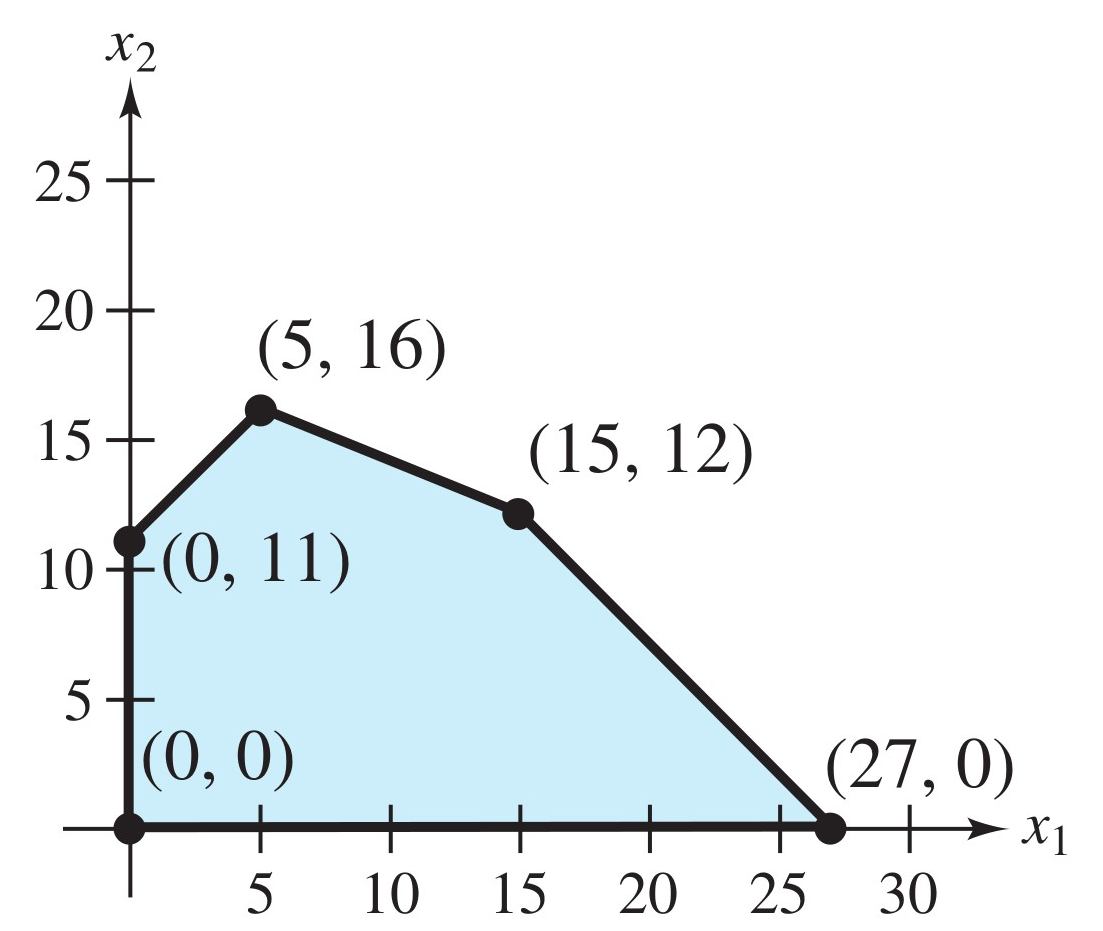
\includegraphics[scale=.2]{LP_region.png}
\end{center}

El conjunto de puntos del plano para los cuales la función toma un valor fijo $z_0$ es una recta
$$
l(z_0) = \{(x_1, x_2) : 4x_1 + 6x_2 = z_0\}.
$$

Geométricamente, si variamos el valor de $z_0$, estamos desplazando la recta obteniendo siempre rectas paralelas. En este caso particular, vemos que si desplazamos la recta hacia arriba, el valor de $z_0$ aumenta, mientras que si desplazamos la recta hacia abajo, el valor de $z_0$ disminuye.

Por lo tanto, podemos resolver el problema gráficamente, desplazando la recta hacia arriba todo lo que podamos mientras que la intersección de la recta con la figura sea no vacía.

Mediante esta resolución gráfica, podemos observar algunas propiedades del problema de programación lineal. Si la región de puntos que satisfacen las restricciones es acotada, forma un polígono, y el óptimo de la función a optimizar se alcanza en el borde del polígono. Más precisamente en un vértice del polígono (puede suceder que el óptimo se alcance también sobre todo un lado del polígono). En particular, dado que un polígono tiene una cantidad finita de vértices, el problema de programación lineal puede resolverse algorítmicamente evaluando la función objetivo sobre todos los vértices del polígono.

Estudiamos ahora el problema en mayor generalidad. Para escribir una combinación lineal de variables vamos a utilizar la notación de producto interno
$$\inner{\cb}{\xb} = c_1 x_1 + \dots + c_n x_n,$$
para $\cb, \xb \in \R^n$.
Un problema de programaci\'on lineal dado en forma est\'andar puede plantearse de la siguiente forma:
\begin{alignat*}{2}
  & \text{minimizar: } & & \inner{\cb}{\xb} \\
   & \text{sujeto a: } & \quad & \Ab\xb = \bb \\
   & & & \xb \ge 0,
\end{alignat*}
donde $\Ab \in \R^{m \times n}$, $\bb \in \R^m$, $\cb \in \R^n$ y la minimizaci\'on se realiza sobre la variable de decisi\'on $\xb \in \R^n$. La condici\'on $\xb \ge 0$ se interpreta componente a componente, es decir $x_i \ge 0$, $1 \le i \le n$. Vamos a ver que un problema donde las restricciones vienen dadas por desigualdades puede llevarse a forma estándar agregando variables auxiliares apropiadas.

\section{Conjuntos convexos y poliedros}

Comenzamos con algunas definiciones básicas.

\begin{definition}~
Dado un vector no-nulo $\ab \in \R^n$ y un escalar $b$,
  \begin{enumerate}
  \item el conjunto $\{\xb \in \R^n | \inner{\ab}{\xb} = b\}$ es un \emph{hiperplano},
  \item el conjunto $\{\xb \in \R^n | \inner{\ab}{\xb} \ge b\}$ es un \emph{semiespacio}.
  \end{enumerate}
\end{definition}

Dada una matriz $\Ab \in \R^{m \times n}$ y un vector $\bb \in \R^n$, en la condición $\Ab \xb = \bb$, cada fila $\ab_i$ de $\Ab$ impone la restricción $\inner{\ab_i}{\xb} = b_i$. El conjunto $\{\xb \in \R^n | \Ab \xb = \bb\}$ corresponde por lo tanto a una intersección de hiperplanos, que llamamos \emph{espacio afín}. Igualmente, en la condición $\Ab \xb \ge \bb$, cada fila $\ab_i$ de $\Ab$ impone la restricción $\inner{\ab_i}{\xb} \ge b_i$ y el conjunto $\{\xb \in \R^n | \Ab \xb \ge \bb\}$ corresponde a una intersección de semiespacios.

\begin{definition}
Un conjunto $S \subset \R^n$ es convexo si para todos $\xb, \yb \in S$, el segmento con vértices $\xb$ e $\yb$ está incluido en $S$. Es decir, para todo $\lambda \in [0, 1]$,
$$
\lambda \xb + (1-\lambda) \yb \in S.
$$
\end{definition}


Dado un problema de programación lineal
\begin{alignat*}{2}
  & \text{minimizar: } & & \inner{\cb}{\xb} \\
   & \text{sujeto a: } & \quad & \Ab\xb = \bb \\
   & & & \xb \ge 0,
\end{alignat*}
podemos interpretar geom\'etricamente el conjunto factible (\emph{feasible set} en ingl\'es), es decir la regi\'on sobre la que queremos minimizar $\inner{\cb}{\xb}$, como la intersecci\'on de un espacio af\'in (definido por la ecuaci\'on $\Ab\xb = \bb$) y el ortante positivo $\xb \ge 0$. Como los dos conjuntos son convexos y la intersecci\'on de conjuntos convexos es tambi\'en convexa, el conjunto factible resulta convexo.

\begin{definition}
Llamamos \emph{poliedro} a un conjunto definido por igualdades y desigualdades lineales:
$$
P = \{\xb \in \R^n \mid \Ab_1 \xb = \bb_1, \Ab_2 \xb = \bb_2\}.
$$
En el caso de que el conjunto resulte acotado, lo llamamos \emph{pol\'itopo}.
\end{definition}

Como las definiciones var\'ian seg\'un la literatura, es importante recordar entonces que para nosotros un poliedro no  necesariamente es un conjunto acotado.

\begin{ejercicio}
Dado el problema
\begin{alignat*}{2}
  & \text{minimizar: } & & 3 x_1 + 5 x_2 \\
   & \text{sujeto a: } & \quad & x_1 + x_2 = 6 \\
   & & & \xb \ge 0,
\end{alignat*}
graficar el conjunto factible, y resolver el problema.
\end{ejercicio}

\section{Variables de holgura}

Dado el problema de programación lineal
\begin{alignat*}{2}
  & \text{minimizar: } & & \inner{\cb}{\xb} \\
   & \text{sujeto a: } & \quad & \Ab\xb \le \bb \\
   & & & \xb \ge \cero,
\end{alignat*}
podemos convertir el problema a un problema con restricciones de igualdad reemplazando cada desigualdad $\inner{\ab_i}{\xb} \le b_i$ por el par de  restricciones
$$\inner{\ab_i}{\xb} + s_i =  b_i, \quad \quad s_i \ge 0,$$
donde $s_i$ es una nueva variable del problema. Estas nuevas variables se llaman \emph{variables de holgura}.

Obtenemos el problema equivalente con restricciones de igualdad
\begin{alignat*}{2}
  & \text{minimizar: } & & \inner{\cb}{\xb} \\
   & \text{sujeto a: } & \quad & \inner{\ab_1}{\xb} + s_1 = b_1 \\
   &  & \quad & \dots \\
   &  & \quad & \inner{\ab_m}{\xb} + s_m = b_m \\
   & & & \xb \ge \cero, \ssb \ge \cero,
\end{alignat*}
con $\ssb = (s_1, \dots, s_m)$.


\begin{ejercicio}
Dado el problema
\begin{alignat*}{2}
  & \text{minimizar: } & & 3 x_1 + 5 x_2 \\
   & \text{sujeto a: } & \quad & x_1 \le 1 \\
   & & & x_2 \le 1 \\
   & & & \xb \ge 0,
\end{alignat*}
\begin{enumerate}
\item graficar el conjunto factible,
\item convertirlo a un problema con igualdades agregando las variables de holgura necesarias,
\item calcular las coordenadas de los vértices del poliedro en el nuevo problema.
\end{enumerate}
\end{ejercicio}


\section{Puntos extremales, vértices y soluciones factibles básicas}

\noindent Referencia: \cite[Sección 2.2]{Bertsimas1997}.

Ya vimos geométricamente que la solución óptima de un problema de programación lineal se encuentra en una \emph{esquina} de la región factible. Veamos ahora diferentes formas de formalizar la idea de esquina.

\begin{definition}
  Dado un poliedro $P$, un vector $\xb \in P$ es un \emph{punto extremal} de $P$ si no puede escribirse como combinación convexa de dos puntos de $P$ distintos de $\xb$. Es decir, si no existen dos vectores $\yb, \zb \in P$, ambos diferentes de $\xb$, y un escalar $\lambda \in [0, 1]$ tales que $\xb = \lambda \yb + (1-\lambda) \zb$.
\end{definition}

Otra posibilidad es considerar a los puntos que son solución óptima única de un problema de programación lineal.

\begin{definition}
  Dado un poliedro $P \subset \R^n$, un vector $\xb \in P$ es un \emph{vértice} de $P$ si existe $\cb \in \R^n$ tal que
  $$\inner{\cb}{\xb} < \inner{\cb}{\yb}$$
   para todo $\yb \in P$, $\yb \neq \xb$.
\end{definition}

Es decir, $\xb$ es un vértice de $P$ si $P$ está de un lado de un hiperplano que toca a $P$ solo en $\xb$.

Una desventaja de estas definiciones geométricas es que dado un poliedro $P$ definido como intersección de hiperplanos y semiespacios, y un punto $\xb$, no es fácil verificar si se cumplen las definiciones. Veremos a continuación una definición alternativa que podemos verificar fácilmente.

Consideramos un poliedro $P$ definido por igualdades y desigualdades lineales,
$$
\begin{cases}
\inner{\ab_i}{\xb} \ge b_i, & i \in M_1 \\
\inner{\ab_i}{\xb} \le b_i, & i \in M_2 \\
\inner{\ab_i}{\xb} = b_i, & i \in M_3,
\end{cases}
$$
donde $M_1, M_2, M_3$ son conjuntos finitos de índices, $\ab_i$ son vectores en $\R^n$ y $b_i$ son escalares.

\begin{definition}
Si un vector $\xb^\star$ satisface una igualdad $\inner{\ab_i}{\xb} = b_i$ para alg\'un $i \in M_1$, $M_2$ o $M_3$, decimos que la condición correspondiente está \emph{activa} en $\xb^\star$.
\end{definition}

Si hay $n$ condiciones activas, $\xb^\star$ es solución de un sistema de $n$ ecuaciones con $n$ incógnitas. Si las $n$ ecuaciones son linealmente independientes, el sistema tiene solución única. Teniendo esto en cuenta, hacemos la siguiente definición.

\begin{definition}
Sean un poliedro $P$ definido por restricciones de igualdades y desigualdades lineales y $\xb^\star \in \R^n$.
\begin{enumerate}
\item El vector $\xb^\star$ es una \emph{solución básica} si
\begin{enumerate}
\item todas las igualdades están activas,
\item de todas las restricciones activas, hay $n$ de ellas que son linealmente independientes
\end{enumerate}
\item Si $\xb^\star$ es una solución básica que satisface todas las restricciones, decimos que $\xb^\star$ es una \emph{solución básica factible}.
\end{enumerate}
\end{definition}

Observamos que en el conjunto de restricciones podemos reemplazar una igualdad $\inner{\ab}{\xb} = b$ por dos desigualdades $\inner{\ab}{\xb} \le b$ y $\inner{\ab}{\xb} \ge b$, obteniendo un problema equivalente. Por lo tanto, la condición de ser solución básica depende de cómo está formulado el problema.

Vimos hasta ahora tres formas de capturar el mismo concepto: punto extremal, vértice y solución básica factible. Veamos ahora que las tres definiciones son equivalentes.

\begin{theorem}
Dado un poliedro $P$ no vacío y un vector $\xb^\star \in P$, las siguientes propiedades son equivalentes:
\begin{enumerate}
\item $\xb^\star$ es un punto extremal de $P$,
\item $\xb^\star$ es un vértice de $P$,
\item $\xb^\star$ es una solución básica factible de $P$.
\end{enumerate}
\end{theorem}

\begin{proof}
Por simplicidad suponemos que el poliedro está definido solo por desigualdades $\inner{\ab_i}{\xb} \ge b_i$ e igualdades $\inner{\ab_i}{\xb} = b_i$.

\textbf{Vértice $\Rightarrow$ Punto extremal.}
Para un vértice $\xb^\star \in P$ , existe $\cb \in \R^n$ tal que $\inner{\cb}{\xb^\star} < \inner{\cb}{\yb}$ para todo $\yb \in P$, $\yb \neq \xb^\star$. Si tomamos $\yb, \zb \in P$, $\yb, \zb \neq \xstar$, y $0 \le \lambda \le 1$, entonces como $\inner{\cb}{\xstar} < \inner{\cb}{\yb}$ y $\inner{\cb}{\xstar} < \inner{\cb}{\zb}$, tenemos que
$$
\inner{\cb}{\xb^\star} < \inner{\cb}{(\lambda \yb + (1-\lambda) \zb)}
$$
y por lo tanto $\xb^\star \neq \lambda \yb + (1-\lambda) \zb$.

\textbf{Punto extremal $\Rightarrow$ Solución básica factible.}
Supongamos que $\xstar \in P$ no es una solución básica factible. Vamos a ver que $\xstar$ no puede ser un punto extremal de $P$. Como $\xstar \in P$ es un punto factible, entonces $\xstar \in P$ no es solución básica. Tomamos $I = \{i \mid \inner{\ab_i}{\xstar} = b_i\}$, el conjunto de índices de las restricciones activas. Como $\xstar$ no es una solución básica, no hay $n$ vectores linealmente independientes en $\{\ab_i\}_{i \in I}$. Si construimos una matriz $\Ab$ con estos vectores como fila, esta matriz tiene rango menor que $n$ y por lo tanto existe $\db \in \R^n$ tal que $\Ab \db = \cero$, es decir, $\inner{\ab_i}{\db_i} = 0$ para todo $i \in I$.

Para $i \not\in I$, $\inner{\ab_i}{\xb} > b_i$. Tomando $\epsilon$ suficientemente pequeño, los vectores $\yb = \xstar + \epsilon \db$ y $\zb = \xstar - \epsilon \db$ también van a cumplir $\inner{\ab_i}{\yb} > b_i$, $\inner{\ab_i}{\zb} > b_i$. Y por definición de $\db$, para $i \in I$, $\inner{\ab_i}{\yb} = \inner{\ab_i}{\xstar + \epsilon \db} = b_i$ y $\inner{\ab_i}{\zb} = b_i$. Luego $\yb, \zb \in P$ y
$$\xstar = \yb + \zb,$$
por lo tanto $\xstar$ no es un punto extremal.

\textbf{Solución básica factible $\Rightarrow$ Vértice.}
Sea $\xstar$ una solución básica factible y sea $I = \{i \mid \inner{\ab_i}{\xstar} = b_i\}$. Sea $\cb = \sum_{i \in I} \ab_i$. Tenemos
$$
\inner{\cb}{\xstar} =  \sum_{i \in I} \inner{\ab_i}{\xstar} = \sum_{i \in I} b_i.
$$

Más aún, para cualquier $\xb \in P$ y cualquier $i$, se cumple $\inner{\ab_i}{\xb} \ge b_i$ y
$$
\inner{\cb}{\xb}=  \sum_{i \in I} \inner{\ab_i}{\xb} \ge \sum_{i \in I} b_i.
$$

Por lo tanto $\xstar$ es una solución óptima al problema de minimizar $\inner{\cb}{\xb}$ sobre $P$. Para concluir, observamos que la igualdad en la última fórmula se cumple si y solo si $\inner{\ab_i}{\xb} = b_i$ para todo $i \in I$. Como $\xstar$ una solución básica factible, en el conjunto $\{\ab_i\}_{i \in I}$ hay $n$ vectores linealmente independientes y por lo tanto $\xstar$ es la única solución del sistema de ecuaciones $\{\inner{\ab_i}{\xb} = b_i\}_{i \in I}$. Luego $\xstar$ es el único minimizante de $\inner{\cb}{\xb}$ en $P$ y por lo tanto es un vértice de $P$.
\end{proof}


Las dos primeras definiciones son definiciones geométricas y solo dependen del conjunto $P$ y no de las ecuaciones que lo definen. Por la equivalencia, obtenemos que la condición de solución básica factible tampoco depende de las ecuaciones que definen $P$, a diferencia de las soluciones básicas que sí pueden depender.

Obtenemos el siguiente corolario simple pero muy importante.

\begin{coro}
Dado un conjunto finito de restricciones lineales (igualdades o desigualdades), la cantidad de soluciones básicas y soluciones básicas factibles es siempre finita.
\end{coro}

\begin{proof}
Dado un sistema de $m$ igualdades y desigualdades lineales, en una solución básica $\xb^\star$ se cumplen al menos $n$ de las restricciones. A la vez, las restricciones deben ser linealmente independientes, y por lo tanto $\xb^\star$ es el único vector que satisface esas restricciones. Por lo tanto soluciones básicas distintas corresponden a distintos conjuntos de $n$ restricciones. Como la cantidad posible de conjuntos de $n$ restricciones es finita, la cantidad de soluciones básicas también.
\end{proof}

Observamos sin embargo que si bien la cantidad de soluciones básicas es siempre finita, puede ser una cantidad muy grande. Por ejemplo, el cubo
$$
\{\xb \in \R^n \mid 0 \le x_i \le 1, 1 \le i \le n\}
$$
está definido por $2n$ ecuaciones y tiene $2^n$ soluciones básicas factibles.
Esto hace que en la práctica, si bien podemos evaluar la función a optimizar en todas las soluciones básicas factibles para encontrar el óptimo, puede ser un método muy ineficiente.

\section{Poliedros en forma estándar}

\noindent Referencia: \cite[Sección 2.3]{Bertsimas1997}

Un poliedro en forma estándar está definido por las siguientes ecuaciones:
$$
P = \{\xb \in \R^n : \Ab\xb = \bb, \xb \ge 0\},
$$
donde $\Ab \in \R^{m \times n}$, es decir el poliedro está definido por $m$ igualdades y $n$ desigualdades $x_i \ge 0$.
Eliminando filas redundantes de $\Ab$, podemos suponer que las $m$ filas de $\Ab$ son linealmente independientes, y por lo tanto debe ser $m \le n$.

Recordemos que en una solución básica debe haber $n$ restricciones linealmente independientes activas, y más aún, todas las restricciones de igualdad se deben cumplir, lo que nos da $m$ restricciones. Como $m \le n$, para obtener $n$ restricciones activas, debemos elegir $n - m$ variables $x_i$ y darles valor $0$, para activar las correspondientes $n-m$ desigualdades $x_i \ge 0$.

Debemos tener cuidado que no cualquier elección de las $n-m$ variables $x_i$ nos va a dar un conjunto de $n$ restricciones linealmente independientes. En el siguiente teorema vemos las condiciones que tenemos que cumplir.

\begin{theorem}
Consideremos las restricciones $\Ab\xb = \bb$ y $\xb \ge 0$, donde suponemos que las $m$ filas de $\Ab \in \R^{m \times n}$ son linealmente independientes.
Un vector $\xb^\star \in \R^n$ es una solución básica si y solo si $\Ab\xb^\star = \bb$ y existen índices $B(1), \dots, B(m)$ tales que
\begin{enumerate}
\item las columnas $\Ab_{B(1)}, \dots, \Ab_{B(m)}$ son linealmente independientes,
\item si $i \neq B(1), \dots, B(m)$, entonces $x_i = 0$.
\end{enumerate}
\end{theorem}

Este teorema nos da un procedimiento para construir soluciones básicas de un poliedro en forma estándar.

\begin{enumerate}
\item Elegir $m$ columnas linealmente independientes $\Ab_{B(1)}, \dots, \Ab_{B(m)}$.
\item Fijar $x_i = 0$ para todo $i \neq B(1), \dots, B(m)$.
\item Resolver el sistema de $m$ ecuaciones $\Ab\xb = \bb$ para las variables $x_{B(1)}, \dots, x_{B(m)}$.
\end{enumerate}

Recordemos que en una matriz el rango fila y el rango columna coinciden, por lo tanto siempre podemos encontrar $m$ columnas independientes en $\Ab$.

Si una solución básica construida siguiendo el procedimiento cumple que todas sus coordenadas son no-negativas, entonces es una solución básica factible. Recíprocamente, podemos encontrar todas las soluciones básicas factibles de esta forma.

Si $\xb$ es una solución básica, llamamos \emph{variables básicas} a las variables $x_{B(1)}, \dots, x_{B(m)}$ y \emph{no-básicas} a las demás variables. Llamamos \emph{columnas básicas} a las columnas $\Ab_{B(1)}, \dots, \Ab_{B(m)}$. Como son linealmente independientes, forman una base de $\R^m$.

Observamos que dos conjuntos distintos de variables básicas pueden dar la misma solución básica, si algunas de las variables básicas valen también $0$. En este caso, decimos que la solución es degenerada. Para simplificar el desarrollo en este apunte, supondremos siempre que todas las soluciones básicas del problema son no-degeneradas.

\section{Existencia de puntos extremales}

En general los poliedros pueden no tener puntos extremales. Por ejemplo, un semiplano en $\R^2$ no tiene puntos extremales.
Una condición muy simple para determinar si un poliedro tiene puntos extremales es la existencia o no de líneas rectas incluidas en el poliedro.

Decimos que un poliedro $P \subset \R^n$ contiene una recta si existe un vector $\xb \in P$ y una dirección $\db \in \R^n$ tales que $\xb + \lambda \db \in P$ para todo $\lambda \in \R$.

\begin{theorem}
Dado un poliedro $P = \{\xb \in \R^n \mid \inner{\ab_i}{\xb} \ge b_i, i = 1, \dots, m\}$, las siguientes condiciones son equivalentes.

\begin{enumerate}
\item El poliedro $P$ contiene al menos un punto extremal.
\item El poliedro $P$ no contiene ninguna recta.
\item Existen $n$ vectores linealmente independientes entre los vectores $\ab_1, \ab_2, \dots, \ab_m$.
\end{enumerate}
\end{theorem}

En particular, cualquier poliedro acotado tiene puntos extremales y cualquier poliedro en forma estándar tiene puntos extremales, debido a que el ortante positivo $\{x_i \ge 0, 1 \le i \le n\}$ no contiene ninguna recta.

Ahora que ya vimos condiciones para que un poliedro tenga puntos extremales, podemos preguntarnos en qué casos un problema de programación lineal tiene soluciones óptimas y verificar que se alcanzan en los puntos extremales, como vimos intuitivamente en los ejemplos.

\begin{theorem}
Consideremos el problema de programación lineal de minimizar una funcional $\inner{\cb}{\xb}$ sobre un poliedro $P$. Si $P$ tiene al menos un punto extremal y el problema tiene solución óptima, entonces existe una solución óptima que es un punto extremal.
\end{theorem}

\begin{proof}
Completar
\end{proof}

Más aún, si el costo óptimo de la función a optimizar es finito, entonces siempre existe solución óptima.

\begin{theorem}
Consideremos el problema de programación lineal de minimizar una funcional $\inner{\cb}{\xb}$ sobre un poliedro $P$. Si $P$ tiene al menos un punto extremal entonces o bien el costo óptimo es $-\infty$ o existe un punto extremal que es óptimo.
\end{theorem}
\begin{proof}
Ver \cite[Teorema 2.8]{Bertsimas1997}
\end{proof}









\section{El método Simplex}

El método Simplex es uno de los métodos más usados en la práctica para resolver problemas de programaci\'on lineal.
A partir de las herramientas desarrolladas en las secciones anteriores, podemos derivar el método simplex en forma sencilla.

Muchos métodos de optimización se basan en un principio simple que consiste en comenzar en una solución factible cualquiera e intentar moverse a otra solución factible cercana de forma que se reduzca el costo de la función a minimizar. Si no existe ninguna solución cercana que permita mejorar la función, hemos alcanzado un mínimo local. En general, un mínimo local no tiene por qué ser un mínimo global, una función podría tener varios mínimos locales, y el mínimo global ser solo uno de ellos.

Afortunadamente, en programación lineal un mínimo local es también global, dado que estamos minimizando una función convexa sobre un conjunto convexo. El método simplex se basa en aprovechar una propiedad adicional de la programación lineal. Ya vimos que en caso de existir un mínimo, este se alcanza en un vértice del poliedro de puntos factibles. Veremos que si estamos parados en un vértice, alcanza verificar si la función objetivo decrece al movernos a alguno de los vértices vecinos (que precisaremos más adelante). Si no decrece en ninguno de los vértices vecinos, hemos encontrado un mínimo local y por lo tanto global.

Obtenemos el siguiente algoritmo
\begin{enumerate}
\item Elegir un vértice $\xb$ del poliedro $P$.
\item Para cada uno de los vértices vecinos $\{\yb_1, \dots, \yb_s\}$ de $\xb$ verificar si la función objetivo mejora en esos puntos.
\item Si no mejora en ninguno de los puntos, $\xb$ es un óptimo global y finalizamos el procedimiento.
\item Si encontramos $\yb_j$ tal que $\inner{\cb}{\yb_j} < \inner{\cb}{\xb}$, tomamos $\xb = \yb_j$ y volvemos a comenzar.
\end{enumerate}

Veremos ahora como obtener los vértices vecinos de un vértice dado, y completaremos los detalles que faltan para probar la correctitud del algoritmo.

Para todo el desarrollo del método simplex, vamos a considerar el problema en forma estándar
\begin{alignat*}{2}
  & \text{minimizar: } & & \inner{\cb}{\xb} \\
   & \text{sujeto a: } & \quad & \Ab\xb = \bb, \\
   & & & \xb \ge 0.
\end{alignat*}



\subsection{Soluciones adyacentes}

Dos soluciones básicas de un conjunto de restricciones lineales en $\R^n$ se dicen \emph{adyacentes} si existen $n-1$ restricciones linealmente independientes que están activas en ambas soluciones. Si las dos soluciones son factibles, llamamos \emph{arista} del conjunto factible al segmento que las une.

\begin{ejercicio}
Sea $P = \{\xb \in \R^n \mid \inner{\ab_i}{\xb} \ge b_i,  1 \le i \le m\}$ un poliedro y $\ub$, $\vb$ dos soluciones básicas factibles adyacentes, con $\inner{\ab_i}{\ub} = \inner{\ab_i}{\vb} = b_i$ para $1 \le i \le n-1$ y $\{\ab_1, \dots, \ab_{n-1}\}$ vectores linealmente independientes.
Probar que el segmento $L = \{\lambda \ub + (1-\lambda)\vb \mid 0 \le \lambda \le 1\}$ que une $\ub$ y $\vb$ verifica
$$
L = \{\zb \in P \mid \inner{\ab_i}{\zb} = b_i, 1\le i \le n-1\}.
$$
\end{ejercicio}

\subsection{Direcciones básicas}

En base a la definición de soluciones adyacentes, para movernos de una solución dada a una adyacente, podríamos reemplazar alguna de las variables básicas por una variable no-básica y calcular la nueva solución básica. Sin embargo, vamos a ver que al elegir cuál es la variable no-básica que vamos a convertir en básica, esto ya determina la dirección en la que debemos movernos para desplazarnos a una solución adyacente.

Sea $\xb$ una solución básica factible de un problema en forma estándar y sean $B(1), \dots, B(m)$ los índices de las variables básicas. Sea $\Bb = [ \Ab_{B(1)} \cdots \Ab_{B(m)}] \in \R^{m \times m}$ la correspondiente matriz base. En particular $x_i = 0$ para cada variable no-básica y  podemos calcular las coordenadas correspondientes a variables básicas por la fórmula
$$
\xb_B = \Bb^{-1}\bb.
$$

Para movernos a una solución adyacente en la que una variable no-básica $x_j$ pase a ser variable básica, debemos desplazarnos a un nuevo vector $$\xb + \theta \db$$
con $\theta > 0$ y $\db = (d_1, \dots, d_n)$ con $d_j =1$ y $d_i = 0$ para todos los índices $i$ distintos de $j$ de variables no-básicas. El vector $\xb_B$ de variables básicas va a cambiar a $\xb_B + \theta \db_B$ con $\db_B = (d_{B(1)}, \dots, d_{B(m)})$.

Como solo nos interesan las soluciones básicas factibles, debe cumplirse
$$
\Ab(\xb + \theta \db) = \bb,
$$
y como $\xb$ también es factible, $\Ab \xb = \bb$. Por lo tanto debe cumplirse $\Ab \db = \cero$ y esto nos permite calcular $\db_B$. En efecto,
$$
\cero = \Ab \db = \sum_{i=1}^n \Ab_i d_i = \sum_{i=1}^m \Ab_{B(i)} d_{B(i)} + \Ab_j = \Bb \db_B + \Ab_j,$$
donde $\Ab_i$ es la $i$-ésima columna de $\Ab$.

Como la matriz $\Bb$ es inversible, obtenemos
$$
\db_B = -\Bb^{-1} \Ab_j.
$$

Llamamos al vector $\db$ que acabamos de construir como la $j$-ésima dirección básica. Por construcción, las restricciones de igualdad se van a mantener mientras nos vamos en esta dirección. Para las condiciones de no-negatividad de las variables, recordemos que la variable no-básica $x_j$ aumenta y las demás variables no-básicas se mantienen en 0, por lo tanto conservan la no-negatividad. Para las variables básicas, como estamos suponiendo que todas las soluciones son no-degeneradas, las variables básicas son todas positivas y podemos tomar $\theta$ suficientemente pequeño para que se sigan cumpliendo.

Antes de calcular el valor de $\theta$ apropiado para movernos a una solución adyacente, calculamos cómo varía el costo de la función a optimizar al desplazarnos en la dirección de la $j$-ésima dirección básica.

Si $\db$ es la $j$-ésima dirección básica, la razón $\inner{\cb}{\db}$ de cambio del costo en la dirección $\db$ está dada por
$$
\inner{\cb}{\db} = \inner{\cb_B}{\db_B} + c_j,
$$
donde $\cb_B = (c_{B(1)}, \dots, c_{B(m)})$. Utilizando que $\db_B = -\Bb^{-1}\Ab_{j}$, hacemos la siguiente definición.

\begin{definition}
Sea $\xb$ una solución básica, sea $\Bb$ la matriz base asociada, y sea $\cb_B$ el vector de costos de las variables básicas. Para cada $j$, definimos el \emph{costo reducido} $\bar c_j$ de la variable $x_j$ por la fórmula
$$
\bar c_j = c_j - \inner{\cb_B}{(\Bb^{-1}\Ab_{j})}.
$$
\end{definition}

El costo reducido nos dice cuánto varía la función de costo al movernos una unidad en la dirección de la $j$-ésima dirección básica. El término $c_j$ indica el aumento del costo por unidad de la variable $x_j$ y el último término es el costo de modificar las demás variables para compensar el cambio en la variable $x_j$.

\begin{example}
\label{ex:simplex}
Consideremos el problema de programación lineal
\begin{alignat*}{2}
  & \text{minimizar: } & & \inner{\cb}{\xb} \\
   & \text{sujeto a: } & \quad & \Ab\xb = \bb \\
   & & & \xb \ge 0,
\end{alignat*}
con $\cb = (2, 0, 0, 0) \in \R^4$,
$$
\Ab = \begin{pmatrix}
1 & 1 & 1 & 1 \\
2 & 0 & 3 & 4
\end{pmatrix} \in \R^{2 \times 4}
\quad \text{ y } \quad \bb = \begin{pmatrix} 2 \\ 2 \end{pmatrix} \in \R^2.
$$

Las primeras dos columnas de $\Ab$ son $\Ab_1 = (1,2)$ y $\Ab_2 = (1, 0)$. Como son linealmente independientes podemos elegir $x_1$ y $x_2$ como variables básicas. La matriz base correspondiente es
$$
\Bb = \begin{pmatrix} 1 & 1 \\ 2 & 0 \end{pmatrix}.
$$

Tomamos $x_3 = x_4 = 0$, y calculamos los valores de $x_1$ y $x_2$: $x_1 = 1$ y $x_2 = 1$. Luego $\xb = (1, 1, 0, 0)$ es una solución básica factible no-degenerada.

Construimos una dirección básica $\db$ correspondiente a aumentar el valor de la variable $x_3$. Tenemos $d_3 = 1$ y $d_4 = 0$. Las coordenedas de $\db$ correspondientes a las variables básicas las obtenemos por la fórmula
$$
\begin{pmatrix} d_1 \\ d_2 \end{pmatrix} =
\begin{pmatrix} d_{B(1)} \\ d_{B(2)} \end{pmatrix} =
\db_B = -\Bb^{-1} \Ab_3 =
-\begin{pmatrix} 0 & 1/2 \\ 1 & -1/2 \end{pmatrix}
\begin{pmatrix} 1 \\ 3 \end{pmatrix} =
\begin{pmatrix} -3/2 \\ 1/2 \end{pmatrix}.
$$

Por lo tanto $\db = (-3/2, 1/2, 1, 0)$ y el costo de movernos en esta dirección es
$$\bar c_3 = \inner{\cb}{\db} = -\frac{3}{2} c_1 + \frac{1}{2}c_2 + c_3 = -3.$$
\end{example}


El siguiente resultado confirma la idea intuitiva que tenemos de los costos reducidos.

\begin{theorem}
Sea $\xb$ una solución básica factible asociada a una matriz base $\Bb$, y sea $\bar \cb$ el vector de costos reducidos.
\begin{enumerate}
\item Si $\bar \cb \ge 0$, entonces $\xb$ es una solución óptima.
\item Si $\xb$ es una solución óptima no-degenerada, entonces $\bar \cb \ge 0$.
\end{enumerate}
\end{theorem}

\begin{proof}\leavevmode
\begin{enumerate}
\item Suponemos $\bar \cb \ge 0$, y consideramos una solución básica factible $\yb$ arbitraria (es decir, $\yb$ es un punto arbitrario del poliedro, no necesariamente un vértice). Definimos $\db = \yb - \xb$. Como $\xb$ e $\yb$ son factibles, $\Ab \xb = \Ab \yb = \bb$ y por lo tanto $\Ab \db = \cero$.

Separando las variables básicas del resto, reescribimos la última igualdad como
$$
\Bb \db_B + \sum_{i \in N} \Ab_i d_i = \cero,
$$
donde $N$ es el conjunto de índices correspondientes a variables no-básicas. Como $\Bb$ es inversible,
$$
\db_B = -\sum_{i \in N} \Bb^{-1} \Ab_i d_i,
$$
y la variación del costo al movernos de $\xb$ a $\yb$ es
\begin{align*}
\inner{\cb}{\yb} - \inner{\cb}{\xb} = \inner{\cb}{\db} &= \inner{\cb_B}{\db_B} + \sum_{i \in N} c_i d_i \\
&= -\inner{\cb_B}{\sum_{i \in N} \Bb^{-1} \Ab_i d_i} + \sum_{i \in N} c_i d_i \\
&= \sum_{i \in N} (c_i - \inner{\cb_B}{(\Bb^{-1} \Ab_i)}) d_i = \sum_{i \in N} \bar c_i d_i.
\end{align*}


Para todo índice no-básico $i \in N$, tenemos $x_i = 0$ y como $\yb$ es factible, $y_i \ge 0$. Por lo tanto, $d_i = y_i - x_i \ge 0$ y $\bar c_i d_i \ge 0$. Concluimos que $\inner{\cb}{\yb} \ge \inner{\cb}{\xb}$ y como $\yb$ era arbitrario, $\xb$ es óptimo.

\item Si $\xb$ es una solución óptima y existe una coordenada $\bar c_j > 0$ del vector de costos reducidos, podemos desplazarnos en la dirección básica correspondiente y reducir el costo, lo que contradice la optimalidad de $\xb$.
\end{enumerate}
\end{proof}

En base a este teorema, para determinar si una solución básica factible no-degenerada es óptima, solo necesitamos chequear si todos los costos reducidos son no-negativos, lo que equivale a examinar si aumenta el costo al movernos en cada una de las $n - m$ direcciones básicas.

Por último, si encontramos una dirección básica en la cual movernos para reducir el costo, debemos calcular el mayor valor de $\theta$ que podemos tomar, lo que equivale a determinar
$$
\theta^\star = \max\{\theta \ge 0 \mid \xb + \theta \db \in P\}.
$$

Vamos a deducir una fórmula para $\theta^\star$. Como $\Ab \db = \cero$, tenemos que
$$
\Ab (\xb + \theta \db) = \Ab \xb = \bb
$$
para todo $\theta$, por lo tanto las restricciones de igual se cumplen siempre. El punto $\xb + \theta \db$ solo puede salirse del poliedro si alguna de las coordenadas se vuelve negativa. Distinguimos dos casos:

\begin{enumerate}
\item Si $\db \ge 0$ (es decir, $d_i \ge 0$ para todo $1 \le i \le n$), entonces $\xb + \theta \db \ge 0$ para todo $\theta \ge 0$. El vector $\xb + \theta \db$ nunca se vuelve no-factible, y tomamos $\theta^\star = +\infty$. El costo óptimo es $-\infty$.

\item Si $d_i < 0$ para algunos $i$, la restricción $x_i + \theta d_i > 0$ nos da la condición
$$
\theta \le -\frac{x_i}{d_i}.
$$
Estas restricciones se deben cumplir para todo $i$ tal que $d_i < 0$. Por lo tanto el mayor valor de $\theta$ que podemos tomar es
\begin{equation*}
\theta^\star = \min_{\{i \mid d_i < 0 \}}\left(-\frac{x_i}{d_i}\right).
\end{equation*}

Recordemos que para las variables $x_i$ no-básicas, o bien $d_i = 1$ si es la variable que pasa a ser variable básica, o bien $d_i = 0$, y en ambos casos $d_i \ge 0$. Por lo tanto podemos restringirnos a mirar las variables básicas en la fórmula anterior. Obtenemos
\begin{equation}
\label{eq:thetastar}
\theta^\star = \min_{\{i = 1, \dots, m \mid d_{B(i)} < 0 \}}\left(-\frac{x_{B(i)}}{d_{B(i)}}\right).
\end{equation}

Más aún, como supusimos que todas las soluciones son no-degeneradas, $x_i > 0$ para todas las variables básicas, y por lo tanto obtenemos siempre $\theta^\star > 0$.
\end{enumerate}

\begin{example}
Continuamos el Ejemplo \ref{ex:simplex}.  Obtuvimos $\xb = (1, 1, 0, 0)$, $\db = (-3/2, 1/2, 1, 0)$ y $\bar c_3 = -3$. Como $\bar c_3$ es negativo, podemos disminuir el costo de la función objetivo desplazándonos en esta dirección. Es decir, consideramos los vectores
$$
\xb + \theta \db,
$$
con $\theta > 0$. La única coordenada que decrece al desplazarnos es $x_1$, por lo que si tomamos cualquier valor de $\theta > 0$ tal que la primera coordenada se mantenga no-negativa, estaremos dentro del poliedro. El máximo valor de $\theta$ que podemos tomar es
$$
\theta^\star = -\frac{x_1}{d_1} = \frac{2}{3},
$$
y nos desplazamos a
$$
\yb = \xb + \frac{2}{3} \db = \left(0, \frac{4}{3}, \frac{2}{3}, 0\right).
$$
Las columnas correspondientes a las coordenadas no-nulas son $\Ab_2 = (1, 0)$ y $\Ab_3 = (1,3)$, y son linealmente independientes. Por lo tanto $\yb$ es una nueva solución básica factible. Como queríamos minimizar el valor de $x_1$, y tenemos la restricción $x_1 \ge 0$, hemos encontrado el costo óptimo. Para verificación, calculamos el costo reducido $\bar c_4$ por la fórmula
$$
\bar c_4 = c_4 - \inner{\cb_B}{(\Bb^{-1} \Ab_4)} = 1 - \begin{pmatrix} 1 & 0 \end{pmatrix} \begin{pmatrix} 1 & 1 \\ 0 & 3 \end{pmatrix}^{-1}
\begin{pmatrix} 1 \\ 4 \end{pmatrix} = \frac{4}{3}.
$$

Vemos que movernos en la dirección básica correspondiente va a incrementar el valor de la función objetivo y por lo tanto no debemos desplazarnos en esa dirección.
\end{example}



Una vez que determinamos $\theta^\star$, suponiendo que es finito, nos movemos a una nueva solución factible
$$
\yb = \xb + \theta^\star \db.
$$
Por la construcción que hicimos de $\db$ y $\theta^\star$, si $\ell$ es el índice que minimiza (\ref{eq:thetastar}), se cumple
$$
x_{B(\ell)} = 0 \quad \text{ y } x_j = \theta^\star.
$$

Es decir que $x_j$ reemplaza a $x_{B(\ell)}$ en el conjunto de variables básicas. Obtenemos un nuevo conjunto de índices de las variables básicas $\bar B = \{\bar B(1), \dots, \bar B(m)\}$ definidos por
$$
\bar B(i) = \begin{cases}
B(i), & i \neq \ell,\\
j, &i = \ell.
\end{cases}
$$

Llamamos $\bar \Bb$ a la nueva matriz base, formada por las columnas de $\Ab$ correspondientes a las nuevas variables básicas.

\begin{theorem}\leavevmode
\begin{enumerate}
\item Las columnas $\Ab_{B(i)}$, $i \neq \ell$, y $\Ab_j$ son linealmente independientes y, por lo tanto, $\bar B$ es una matriz base.
\item El vector $\yb = \xb + \theta^\star \db$ es una solución básica factible con matriz base asociada $\bar \Bb$.
\end{enumerate}
\end{theorem}

\begin{proof}
Ver \cite[Teorema 3.2]{Bertsimas1997}.
\end{proof}

Mediante el procedimiento descripto, pasamos de una solución básica factible a otra solución básica factible con menor costo.
Obtenemos la siguiente iteración del método simplex.

\begin{enumerate}[label = (\arabic*)]
\item Comenzamos con una solución básica factible $\xb$, correspondiente a variables básicas con índices $I = \{B(1), \dots, B(m)\}$.
\item Tomamos la submatriz $\Bb$ de $\Ab$ formada por las columnas correspondientes a las variables básicas, y calculamos los costos reducidos $$\bar c_j = c_j - \inner{\cb_B}{(\Bb^{-1} \Ab_j)}.$$
Si todos los costos son no-negativos, $\xb$ es una solución óptima y terminamos. Si no, elegimos algún $j$ tal que $\bar c_j < 0$.
\item Calculamos $\ub = -\db_B = \Bb^{-1} \Ab_j$. Si $\ub$ no tiene ninguna componente positiva, tomamos $\theta^\star = \infty$, el costo óptimo es $-\infty$ y el algoritmo termina.
\item Si alguna componente de $\ub$ es positiva, tomamos
$$
\theta^\star = \min_{\{i = 1, \dots, m \mid u_i > 0\}} \frac{x_{B(i)}}{u_i}.
$$
\item Sea $\ell$ un índice para el cuál se alcanza el mínimo. Construimos una nueva base reemplazando $B(\ell)$ por $j$. La nueva variable básica $\yb$ queda definida por
    $$
    \begin{cases}
    y_j = \theta^\star, \\
    y_{B(i)} = x_{B(i)} - \theta^\star u_i, & 1 \le i \le m, i \neq l \\
    y_i = 0 & \text{ para los índices de variables no-básicas.}
    \end{cases}
    $$
\end{enumerate}

En base a todo lo que vimos es fácil verificar que el método simplex descripto resuelve correctamente el problema de programación lineal.
En particular, esto nos permite demostrar la siguiente propiedad de los problemas de programación lineal.

\begin{theorem}
Consideremos el problema de programación lineal de minimizar una funcional $\inner{\cb}{\xb}$ sobre un poliedro $P$. Si $P$ tiene al menos un punto extremal entonces o bien el costo óptimo es $-\infty$ o existe un punto extremal que es óptimo.
\end{theorem}
%\begin{proof}
%Ver \cite[Teorema 2.8]{Bertsimas1997}
%\end{proof}









\subsection{El tableau del método Simplex}

Veremos ahora una implementación del método simplex utilizando mediante operaciones elementales de filas de una matriz, que suele llamarse \emph{tableau}.

Vamos a verlo en el siguiente ejemplo concreto:
\begin{alignat*}{2}
   & \text{maximizar: } \quad &  4 x_1 + 6 x_2 &= z\\
   & \text{sujeto a: }  \quad & -x_1 + x_2 &\le 11 \\
   &   \quad & x_1 + x_2 &\le 27 \\
   &   \quad & 2x_1 + 5x_2 &\le 90 \\
   & &  \xb &\ge 0.
\end{alignat*}

Como tenemos todas desigualdades menor o igual, agregamos variables de holgura $s_1$, $s_2$, $s_3$ y reemplazamos las desigualdades por igualdades:
\begin{alignat*}{2}
   & \text{maximizar: } \quad &  4 x_1 + 6 x_2 &= z\\
   & \text{sujeto a: }  \quad & -x_1 + x_2 +s_1&= 11 \\
   &   \quad & x_1 + x_2 +s_2&= 27 \\
   &   \quad & 2x_1 + 5x_2 +s_3&= 90 \\
   & &  \xb, \ssb &\ge 0.
\end{alignat*}

Como ya vimos, una \emph{solución básica} de un problema en forma estándar es una solución
$$(x_1, x_2, \dots, x_n, s_1, s_2, \dots, s_m)$$
 en la que \emph{a lo sumo} $m$ variables son nulas. Las variables no-nulas se llaman \emph{variables b\'asicas} de la solución. Si todas las variables son no-negativas, la solución se llama \emph{solución básica factible}.

La matriz inicial del método se construye colocando todas las ecuaciones de restricciones como filas, y una última fila con los coeficientes de la función objetivo escrita de la siguiente forma:
$$
-c_1 x_1 - c_2 x_2 - \dots - c_n x_n + 0 s_1 + \dots + 0 s_m + z = 0.
$$
En general omitimos el coeficiente de $z$ que se mantiene siempre en 1.

En el ejemplo, obtenemos el tableau
$$
\begin{array}{ccccccc}
x_1 & x_2 & s_1 & s_2 & s_3 & b & \\ \hline
-1 & 1 & 1 & 0 & 0 & 11 & s_1 \\
1 & 1 & 0 & 1 & 0 & 27 & s_2 \\
2 & 5 & 0 & 0 & 1 & 90 & s_3 \\ \hline
-4 & -6 & 0 & 0 & 0 & 0 &
\end{array}
$$

Las variables básicas al comenzar son $s_1, s_2, s_3$ y las variables $x_1$ y $x_2$ comienzan con valor $0$.

La solución básica inicial es
$$
x_1 = 0, x_2 = 0, s_1 = 11, s_2 = 27, s_3 = 90
$$
que en este caso resulta una solución básica factible.

En este momento podemos verificar si la solución que tenemos es óptima. La condición del método simplex para una solución óptima es que todos los números en la última fila sean no-negativos. En nuestro caso, tenemos dos coeficientes negativos y por lo tanto la solución no es óptima.

\subsubsection{Pivoteo}
Como la solución no es óptima, realizamos operaciones de pivoteo para obtener en sucesivos pasos mejores soluciones hasta llegar a la solución óptima.

Elegimos una nueva variable básica, que va a reemplazar a alguna de las variables básicas actuales.
Definimos
\begin{itemize}
\item Variable entrante a la variable con el menor valor (el más negativo) en la última fila, que tomamos como nueva variable básica.
\item Variable saliente a la variable con menor cociente $b_i / a_{ij}$ en la columna determinada por la variable entrante.
\item El pivot es la casilla de la matriz en la columna de la variable entrante y la fila de la variable saliente.
\end{itemize}

Finalmente, realizamos eliminación de Gauss-Jordan por filas sobre toda la matriz, tomando el pivot recién definido.

En nuestro ejemplo, la variable entrante es $x_2$ y la variable saliente es $s_1$.

Observaciones:
\begin{itemize}
\item La operación de pivoteo se corresponde con aumentar el valor de alguna de las variables que tenían valor 0. La elección de la variable entrante se hace de forma tal que un cambio en esta variable produzca un cambio mayor que el de las otras variables.
\item Para elegir la variable saliente, buscamos cuál es el máximo valor que podemos darle a la variable entrante sin violar las restricciones. En nuestro ejemplo, el mayor valor es $x_2 = 11$. Este valor nos permite encontrar soluciones factibles $(x_1, x_2)$ para las 3 restricciones. Si le diéramos un valor mayor, se violaría la primera restricción.
\end{itemize}

Al realizar el pivoteo, obtenemos el tableau
$$
\begin{array}{ccccccc}
x_1 & x_2 & s_1 & s_2 & s_3 & b & \\ \hline
-1 & 1 & 1 & 0 & 0 & 11 & x_2 \\
2 & 0 & -1 & 1 & 0 & 16 & s_2 \\
7 & 0 & -5 & 0 & 1 & 35 & s_3 \\ \hline
-10 & 0 & 6 & 0 & 0 & 66 &
\end{array}.
$$

Vemos que obtuvimos una solución mejorada
$$
(x_1, x_2, s_1, s_2, s_3) = (0, 11, 0, 16, 35)
$$
y el valor de la función objetivo es
$$
4 x_1 + 6 x_2 = 66.
$$

Esta solución no es óptima porque $x_1$ tiene signo negativo en la ultima fila, podemos aumentar el valor de $x_1$.

Tomamos $x_1$ como variable saliente y calculando los cocientes, tomamos $s_3$ como variable saliente.

Al aplicar Gauss-Jordan obtenemos
$$
\begin{array}{ccccccc}
x_1 & x_2 & s_1 & s_2 & s_3 & b & \\ \hline
0 & 1 & 2/7 & 0 & 1/7 & 16 & x_2 \\
0 & 0 & 3/7 & 1 & -2/7 & 6 & s_2 \\
1 & 0 & -5/7 & 0 & 1/7 & 5 & s_3 \\ \hline
0 & 0 & -8/7 & 0 & 10/7 & 116 &
\end{array}.
$$

Esta solución no es óptima porque $s_3$ tiene signo negativo en la ultima fila, podemos aumentar el valor de $s_3$.
Tomando $s_3$ como variable entrante y $s_2$ como variable saliente, obtenemos luego de pivotear:
$$
\begin{array}{ccccccc}
x_1 & x_2 & s_1 & s_2 & s_3 & b & \\ \hline
0 & 1 & 0 & -2/3 & 1/3 & 12 & x_2 \\
0 & 0 & 1 & 7/3 & -2/3 & 14 & s_2 \\
1 & 0 & 0 & 5/3 & -1/3 & 15 & x_1 \\ \hline
0 & 0 & 0 & 8/3 & 2/3 & 132 &
\end{array}.
$$


Encontramos la solución óptima del problema
$$
(x_1, x_2, s_1, s_2, s_3) = (15, 12, 0, 14, 0)
$$
con valor de la función objetivo
$$
4 x_1 + 6 x_2 = 132.
$$







\section{El problema dual}

\noindent Referencia principal: \cite[Capítulo 4]{Bertsimas1997}.

Una de las propiedades m\'as interesantes de la programaci\'on lineal es que a cada problema primal en forma estándar
\begin{alignat*}{2}
  & \text{maximizar: } & & \inner{\cb}{\xb}  \\
   & \text{sujeto a: } & \quad & \Ab \xb = \bb, \\
   &&& \xb \ge 0
\end{alignat*}
podemos asociarle un problema dual de la siguiente forma:
\begin{alignat*}{2}
  & \text{maximizar: } & & \inner{\yb}{\bb}  \\
   & \text{sujeto a: } & \quad & \Ab^T \yb \le \cb, \\
\end{alignat*}
que guarda relaciones muy fuertes con el problema primal.

\subsection{Motivación}

Consideremos el problema en forma estándar
\begin{alignat*}{2}
  & \text{minimizar: } & & \inner{\cb}{\xb}  \\
   & \text{sujeto a: } & \quad & \Ab \xb = \bb \\
   & & & \xb \ge 0,
\end{alignat*}
que llamamos \emph{problema primal}, y notamos $\xb^\star$ a una solución óptima que suponemos que existe.

Podemos relajar este problema reemplazando la restricción $\Ab\xb = \bb$ por una penalidad $\inner{\yb}{(\bb - \Ab\xb)}$, donde $\yb$ es un vector de precios del mismo tamaño que $\bb$. Obtenemos entonces el siguiente problema:
\begin{alignat*}{2}
  & \text{minimizar: } & & \inner{\cb}{\xb} + \inner{\yb}{(\bb - \Ab\xb)}, \\
   & \text{sujeto a: } & \quad & \xb \ge \cero.
\end{alignat*}

Llamamos $g(\yb)$ al costo óptimo en función de $\yb$ del problema relajado. Como tenemos más libertad en la elección de variables en el problema relajado, esperamos que $g(\yb)$ sea menor o igual que el costo óptimo $\inner{\cb}{\xb^\star}$ del problema primal. En efecto,
$$
g(\yb) = \min_{\xb \ge 0} \left\{ \inner{\cb}{\xb} + \inner{\yb}{(\bb-\Ab\xb)}\right\} \le \inner{\cb}{\xb^\star} + \inner{\yb}{(\bb - \Ab\xb^\star)} = \inner{\cb}{\xb^\star},
$$
donde usamos para la última desigualdad que $\xb^\star$ es una solución óptima del problema primal y por lo tanto $\Ab\xb^\star = \bb$.

Por lo tanto, para cualquier vector $\yb$, $g(\yb) \le \inner{\cb}{\xb^\star}$ y el valor de $g(\yb)$ es una cota inferior del costo óptimo $\inner{\cb}{\xb^\star}$ del problema primal. Queremos hallar la mejor cota posible, es decir, queremos hallar el vector $\yb$ que maximice $g(\yb)$. Este problema se conoce como el \emph{problema dual}, que podemos plantear en la forma:
\begin{alignat*}{2}
  & \text{maximizar: } & & g(\yb), \\
   & \text{sujeto a: } & \quad & \text{ninguna restricción}.
\end{alignat*}

El resultado principal de la teoría de dualidad afirma que el costo óptimo del problema dual es igual al costo óptimo $\inner{\cb}{\xb^\star}$ del problema primal. En otras palabras, si elegimos el valor de $\yb$ para el cual $g(\yb)$ es máximo, la posibilidad de violar las restricciones $ \Ab\xb = \bb$ no es de ninguna ayuda.

Por la definición de $g(\yb)$,
$$
\begin{aligned}
g(\yb) = \min_{\xb \ge 0} \left\{ \inner{\cb}{\xb} + \inner{\yb}{(\bb-\Ab\xb)}\right\}
&= \inner{\yb}{\bb} + \min_{\xb \ge 0} \left\{ \inner{\cb}{\xb} - \inner{\yb}{(\Ab\xb)} \right\} \\
&= \inner{\yb}{\bb} + \min_{\xb \ge 0} \left\{ \inner{\cb}{\xb} - \inner{(\Ab^T\yb)}{\xb} \right\} \\
&= \inner{\yb}{\bb} + \min_{\xb \ge 0} \left\{ \inner{(\cb - \Ab^T\yb)}{\xb} \right\},
\end{aligned}
$$
recordando que $\inner{\xb}{(\Ab\yb)} = \xb^T \Ab \yb = (\Ab^T \xb)^T \yb = \inner{(\Ab^T \xb)}{\yb}$.

Ahora bien, notemos que
$$\min_{\xb \ge 0} \left\{ \inner{(\cb - \Ab^T\yb)}{\xb} \right\} = \begin{cases}
0 & \text{si } \cb - \Ab^T\yb \ge \cero, \\
-\infty, & \text{en otro caso.}\end{cases}
$$

Como queremos maximizar $g(\yb)$, podemos quedarnos solo con los casos para los que $g(\yb) \neq -\infty$. Concluimos que el problema dual es equivalente al problema
\begin{alignat*}{2}
  & \text{maximizar: }  & \quad & \inner{\yb}{\bb},   \\
   & \text{sujeto a: }  &       & \Ab^T\yb \le \cb. \\
\end{alignat*}

En resumen, definimos un vector $\yb$ de parámetros o variables duales, y para cada elección de $\yb$ podemos encontrar una cota inferior para costo óptimo del problema primal. El problema dual consiste en maximizar esa cota, es decir, obtener la cota mas precisa posible. Para algunos vectores $\yb$, la cota que obtenemos es $-\infty$, que no tiene utilidad. Por lo tanto, nos restringimos a las elecciones de $\yb$ que nos dan cotas no triviales, y eso nos da las restricciones del problema dual.

\subsection{Teoremas de dualidad débil y fuerte}

A partir del razonamiento anterior, deducimos el siguiente resultado

\begin{theorem}[Dualidad débil]
Si $\xb$ es una solución factible del problema primal y $\yb$ es una solución factible del problema dual, entonces
$$
\inner{\yb}{\bb} \le \inner{\cb}{\xb}.
$$
\end{theorem}

Si bien este resultado es muy simple, tiene consecuencias interesantes.

\begin{coro}~
\begin{itemize}
\item Si el costo óptimo del problema primal es $-\infty$, entonces el problema dual no es factible.
\item Si el costo óptimo del problema dual es $+\infty$, entonces el problema primal no es factible.
\end{itemize}
\end{coro}


\begin{coro}
Sean $\xb^\star \in \R^n$ e $\yb^\star \in \R^m$ soluciones factibles de los problemas primal y dual respectivamente, y supongamos que $\inner{\yb^\star}{\bb} = \inner{\cb}{\xb^\star}$. Entonces $\xb^\star$ y $\yb^\star$ son soluciones óptimas de los problemas primal y dual respectivamente.
\end{coro}

Enunciamos ahora el resultado principal de la teoría dual de programación lineal.

\begin{theorem}[Dualidad fuerte]
Si un problema primal de programación lineal tiene solución óptima, entonces también el problema dual tiene solución óptima, y los respectivos costos óptimos son iguales.
\end{theorem}

\begin{proof}
  Si aplicamos el método Simplex al problema primal
\begin{alignat*}{2}
  & \text{minimizar: } & \quad & \inner{\cb}{\xb}  \\
  & \text{sujeto a: }   & & \Ab \xb = \bb \\
  & & & \xb \ge 0,
\end{alignat*}
vamos a obtener una solución óptima $\xb$ con base $\Bb$. Tomamos $\xb_B = \Bb^{-1}\bb$ el vector de los valores óptimos de las variables básicas.
El vector de costos reducidos es
$$\cb^T - \cb_B^T \Bb^{-1} \Ab,$$
donde $\cb_B^T$ es el vector de costos (coeficientes) de las variables básicas.
Como $\xb$ es una solución óptima,
$$\cb^T - \cb_B^T \Bb^{-1} \Ab \ge 0.$$

%($\pb^T = \cb_B^T \Bb^{-1}$)
Definimos ahora $\yb \in \R^m$ tal que $\yb^T = \cb_B^T \Bb^{-1}$. Vemos que $\yb^T \Ab  \le \cb^T$, o equivalentemente $\Ab^T \yb \le \cb$, y por lo tanto $\yb$ es una solución factible del problema dual
\begin{alignat*}{2}
  & \text{maximizar: } & \quad  & \inner{\yb}{\bb} \\
  & \text{sujeto a: }  & & \Ab^T \yb \le \cb.
\end{alignat*}

Más aún,
$$
\inner{\yb}{\bb} = \inner{(\Bb^{-1})^T \cb_B}{\bb} = \inner{\cb_B}{\Bb^{-1} \bb} = \inner{\cb_B}{\xb_B} = \inner{\cb}{\xb}.
$$
Por lo tanto, por dualidad débil, $\yb$ es una solución optima del problema dual y el costo óptimo dual coincide con el costo óptimo primal.
\end{proof}



%Veamos un ejemplo.
%
%\begin{example}
%Consideramos el problema
%\begin{align*}
%   \text{minimizar: } &  x_1 - 8 x_2 \\
%    \text{sujeto a: } & \left\{
%   \begin{array}{rcl}
%   -x_1 + 3x_2 + x_3 & = & 4, \\
%   4x_1 -  x_2 + x_4 & = & 6, \\
%   \xb & \ge &  0.
%   \end{array}
% \right.
%\end{align*}
%
%El conjunto factible es un poliedro de 2 dimensiones en $\R^4$. Como estamos minimizando una funci\'on que depende solo de las dos primeras variables, podemos proyectar este conjunto en el plano $(x_1, x_2)$. Obtenemos el pol\'igono de la Figura 2.1.
%
%Para resolver el problema, graficamos la recta $x_1-8x_2 = 0$. Sobre todos los puntos en esa recta, la funci\'on objetivo toma el valor $0$. Anal\'ogamente, si trazamos una recta paralela, la funci\'on objetivo tomar\'a un valor constante en esa recta. Si la recta se desplaza hacia la derecha el valor de la funci\'on aumentar\'a y si la desplazamos hacia la izquierda el valor disminuir\'a.
%Por lo tanto, debemos desplazarla hacia la izquierda todo lo que sea posible sin que haya interesecci\'on vac\'ia entre la recta y el pol\'igono.  Concluimos que el m\'inimo se alcanza en el punto $(x_1, x_2) = (2,2)$ y resolviendo los valores de $x_3$ y $x_4$ obtenemos que el m\'inimos es $\xb^\star = (2,2,0,0)$.
%
%
%\end{example} 
\chapter{Introducci\'on a la programaci\'on semidefinida}

\section{Motivación}
Consideremos una sucesión de vectores definida recursivamente por
$$
x[k + 1] = A x[k], \quad x[0] = x_0
$$

Se puede ver que este sistema tiende a 0 para todo vector inicial si y solo todos los autovalores de $A$ tienen módulo menor que 1.
En este caso entonces, para estudiar el comportamiento en el largo plazo del sistema, nos interesa conocer el máximo de los módulos de los autovectores de $A$, que llamamos \emph{radio espectral} de $A$.

Dada una matriz $A$ con autovalores $\lambda_1, \dots, \lambda_n$, los autovalores de $A - \alpha I$ son $\lambda_1 - \alpha, \dots, \lambda_n - \alpha$. SI $A$ es simétrica, todos sus autovalores son reales, y podemos calcular su radio espectral calculando el mayor y menor autovalor.

En este caso, podemos plantear el problema de hallar el menor autovalor como un problema de optimización:
$$
\min \{\lambda : \lambda \text{ autovalor de $A$}\} = \sup_{\alpha \in \R} \{\alpha : A - \alpha I \succeq 0\}
$$
y análogamente, podemos plantear el problema de hallar el mayor autovalor como
$$
\max \{\lambda : \lambda \text{ autovalor de $A$}\} = \inf_{\alpha \in \R} \{\alpha : \alpha I - A \succeq 0\}.
$$

Estudiaremos cómo resolver este tipo de problemas.

\section{Preliminares}

\subsection{Matrices simétricas}

Notamos $\Sym^n$ al espacio de matrices simétricas
$$
\Sym^n = \{A \in \R^{n \times n} | a_{ij} = a_{ji}, \forall 1 \le i, j \le n\}.
$$
Es un subespacio vectorial de $\R^{n \times n}$ de dimensión $\frac{n(n+1)}{2}$.

Una propiedad fundamental de las matrices simétricas es que todos los autovalores son reales, y poseen base ortonormal de autovectores.
Este resultado se conoce como el teorema espectral.

\begin{prop}
Si $\Ab$ es simétrica, entonces
\begin{enumerate}
\item \label{item:realav} todos los autovalores de $\Ab$ son reales,
\item autovectores correspondientes a autovalores distintos son perpendiculares,
\item $\Sb^T \Ab \Sb$ es simétrica para toda $\Sb \in \Rnn$.
\end{enumerate}
\end{prop}

\begin{proof}
Ejercicio.
\end{proof}

\begin{theorem}
Cualquier matriz simétrica $X \in \Symn$ admite una descomposición
$$
X = P D P^T,
$$
con $P \in \Rnn$ matriz ortogonal y $D \in \Rnn$ matriz diagonal, con los autovalores $\{\lambda_1, \dots, \lambda_n\} \subset \R$ de $X$ en la diagonal. Equivalentemente,
$$
X = \sum_{i=1}^n \lambda_i u_i u_i^T,
$$
con $u_i \in \R_n$, $1 \le i \le n$, los autovectores de $X$, que se corresponden con las columnas de $P$.
\end{theorem}

\begin{proof} Ver \cite[Teorema 4.1.5]{Horn1985}.
\end{proof}

\subsection{Matrices simétricas y ley de inercia}

En el caso de matrices simétricas existe una diagonalización más simple que la diagonalización por matrices semejantes, que es especialmente útil en problemas de programación semidefinida.

\begin{definition}
Dos matrices $A, B \in \Rnn$ son \emph{congruentes} si existe una matrix $S \in \Rnn$ inversible tal que
$$
A = S B S^T.
$$
\end{definition}

La relación de congruencia es una relación de equivalencia.

Dada una matriz simétrica $\Ab \in \Symn$ definimos la \emph{inercia} de $\Ab$ como la terna $(n_+, n_-, n_0)$, donde $n_+$ la cantidad de autovalores positivos, $n_-$ la cantidad de autovalores negativos y $n_0$ es la cantidad de autovalores nulos de $\Ab$.

Si $\Ab \in \Symn$, podemos escribir $\Ab = \Ub \Lambdab \Ub^T$ con $\Lambda = \diag(\lambda_1, \dots, \lambda_n)$, la matriz con los autovalores de $\Ab$ en la diagonal, y $\Ub$ unitaria. Suponemos que los autovalores positivos son los primeros, luego los autovalores negativos y finalmente los autovalores cero. Definiendo la matriz diagonal no-singular real
$$\Db = \diag(\sqrt{\lambda_1}, \dots, \sqrt{\lambda_{n_+}}, \sqrt{-\lambda_{n_{+}+1}}, \dots, \sqrt{-\lambda_{n_{+}+n_{-}}}, 1, \dots, 1),$$
obtenemos
$$
\Lambda = D \begin{pmatrix}
1 &        &   &    &        &    &   &        &   \\
  & \ddots &   &    &        &    &   &        &   \\
  &        & 1 &    &        &    &   &        &   \\
  &        &   & -1 &        &    &   &        &   \\
  &        &   &    & \ddots &    &   &        &   \\
  &        &   &    &        & -1 &   &        &   \\
  &        &   &    &        &    & 0 &        &   \\
  &        &   &    &        &    &   & \ddots &   \\
  &        &   &    &        &    &   &        & 0 \\
\end{pmatrix}
D.$$

Podemos escribir a la matriz $\Ab$ como
$$
\Ab = \Ub \Lambda \Ub^T = \Sb
\begin{pmatrix}
1 &        &   &    &        &    &   &        &   \\
  & \ddots &   &    &        &    &   &        &   \\
  &        & 1 &    &        &    &   &        &   \\
  &        &   & -1 &        &    &   &        &   \\
  &        &   &    & \ddots &    &   &        &   \\
  &        &   &    &        & -1 &   &        &   \\
  &        &   &    &        &    & 0 &        &   \\
  &        &   &    &        &    &   & \ddots &   \\
  &        &   &    &        &    &   &        & 0 \\
\end{pmatrix}
\Sb^T = S I(A) S^T,$$
donde $\Sb = \Ub \Db$ es una matriz no-singular y $I(A)$ es la matriz de inercia de $\Ab$.

Utilizando esta escritura, la ley de inercia nos permite determinar fácilmente si dos matrices simétricas son congruentes.

\begin{theorem}
Dos matrices simétricas $A, B \in \Symn$ son congruentes si y solo si tienen la misma signatura.
\end{theorem}

\begin{proof}
Si dos matrices $\Ab, \Bb$ tienen la misma inercia, utilizando la construcción anterior, obtenemos que $\Ab$ y $\Bb$ son congruentes a la misma matriz de inercia. Como la relación de congruencia es una relación de equivalencia, las matrices $\Ab$ y $\Bb$ son congruentes.

Para la otra implicación, suponemos $\Ab$ y $\Bb$ congruentes, con $\Ab = \Sb \Bb \Sb^T$, para alguna matriz no-singular $\Sb \in \Rnn$. Como las matrices congruentes tienen el mismo rango, $n_0(\Ab) = n_0(\Bb)$ y alcanza ver que $n_+(\Ab) = n_+(\Bb)$. Notamos $k = n_+(\Ab)$.

Sean $\vb_1, \dots, \vb_k$ autovectores ortonormales de $\Ab$ correspondientes a los autovalores positivos $\lambda_1(\Ab), \dots, \lambda_{k}$ y sea $S_+(\Ab) = \langle \vb_1, \dots, \vb_{k} \rangle$.

La dimensión de $S_+(\Ab)$ es $k$, y si
$$\xb = \alpha_1 \vb_1 + \dots + \alpha_k \vb_{k} \neq 0,$$
entonces
$$\xb^T \Ab \xb = \lambda_1(A) |\alpha_1|^2 + \dots + \lambda_{k}(A) |\alpha_k|^2 > 0.$$

Por lo tanto,
$$
\xb^T (\Sb \Bb \Sb^T) \xb = (\Sb^T\xb)^T \Bb (\Sb^T \xb) > 0,
$$
luego $\yb^T \Bb \yb > 0$ para todo vector no nulo $\yb \in \langle \Sb^T \vb_1, \dots, \Sb^T \vb_k \rangle$, que es un espacio de dimensión $k$. Por lo tanto, $n_+(\Bb) \ge k = n_+(\Ab)$ y realizando el mismo razonamiento intercambiando $\Ab$ por $\Bb$, obtenemos $n_+(\Ab) = n_+(\Bb)$.
\end{proof}

En particular, cualquier matriz simétrica es congruente a una matriz diagonal con valores $0$, $+1$ o $-1$ en la diagonal, y la cantidad de cada uno de estos valores en la diagonal es invariante, no depende de la matriz $\Sb$.

Finalmente, notamos que dada una matriz simétrica $\Ab \in \Symn$ podemos obtener una matriz diagonal $\Db$ congruente a $\Ab$ por eliminación gaussiana (realizando simultáneamente eliminación en filas y columnas). Por lo tanto, podemos calcular eficientemente tanto la diagonalización por congruencia como la signatura de la matriz.


\subsection{Matrices definidas positivas}

Una matriz $A \in \R^{n \times n}$ se llama \emph{semidefinida positiva} si es simétrica y
$$
x^T A x  \ge 0
$$
para todo $x \in \R^n$. Si además $x^T A x = 0$ solo para $x = 0$, decimos que la matriz es \emph{definida positiva}.

Si $A = M^T M$ para $M \in \R^{m \times n}$ cualquiera, entonces
$$
x^T A x = x^T M^T M x = \| Mx \|^2 \ge 0,
$$
lo que nos da un amplio stock de matrices positivas semidefinidas.

Para el siguiente resultado, dado un conjunto $S \subset \{1, \dots, n\}$, definimos el menores principales asociado a $S$ como el determinante de la submatriz cuadrada  $A_{S,S}$ formada por las filas y columnas de $A$ con índices en $S$.
SI $S = \{1, 2, \dots, k\}$, decimos que el menor asociado es un \emph{menor principal de cabeza}.

\begin{theorem}
  Si $A \in \Rnn$ es un matriz simétrica, las siguientes propiedades son equivalentes.
  \begin{enumerate}
  \item $A$ es semidefinida positiva ($x^T A x \ge 0$ para todo $x \in \R^n$),
  \item $A = M^T M$ para alguna matriz $M \in \R^{n \times n}$,
  \item todos los autovalores de $A$ son no-negativos,
  \item \emph{todos} los menores principales de $A$ son no-negativos.
  \end{enumerate}
\end{theorem}

Para matrices definidas positivas, obtenemos equivalencias similares.

\begin{theorem}
  Si $A \in \Rnn$ es un matriz simétrica, las siguientes propiedades son equivalentes.
  \begin{enumerate}
  \item $A$ es definida positiva ($x^T A x > 0$ para todo $x \in \R^n$),
  \item \label{MTM} $A = M^T M$ para alguna matriz $M \in \R^{n \times n}$ no singular,
  \item todos los autovalores de $A$ son positivos,
  \item \label{menoresprincipales} todos los menores principales de $A$ son positivos,
  \item el polinomio característico de $\Ab$ tiene signos alternados. Si $\chi_A(x) = x^n + a_{n-1} x^{n-1} + a_1 x + a_0$, entonces $a_i a_{i+1} < 0$ para todo $0 \le i \le {n-1}$ (definiendo $a_n = 1$).
  \end{enumerate}
\end{theorem}

En el caso de matrices definidas positivas, podemos restringir la condición \ref{menoresprincipales} a considerar solo los menores principales de cabeza.

En ambos casos, la condición $\ref{MTM}$ podemos restringirla a matrices triangulares inferiores. Recordemos que cualquier matriz $C \in \Rnn$ admite una descomposición $\Qb\Rb$ y puede escribirse como $\Cb = \Qb \Rb$ con $\Qb$ unitaria y $\Rb$ triangular superior del mismo rango que $\Cb$. Luego
$$
\Ab = \Cb^T \Cb = (\Qb \Rb)^T \Qb \Rb = \Rb^T \Qb^T \Qb \Rb = \Rb^T \Rb
$$
y tomando $\Lb = \Rb^T$, obtenemos $\Ab = \Lb \Lb^T$.

Si $\Cb$ es no singular, podemos elegir $\Rb$ con todos los valores en la diagonal positivos (y la descomposición de esta forma es única).
Esto prueba el siguiente corolario, que nos da la \emph{descomposición de Cholesky} de una matriz definida positiva.

\begin{corollary}
Una matriz $\Ab$ es definida positiva si y solo si existe una matriz trinagular inferior $\Lb \in \Rnn$ con valores positivos en la diagonal tal que $\Ab = \Lb \Lb^T$.
\end{corollary}


La siguiente propiedad será clave para estudiar la dualidad en programación semidefinida.

\begin{theorem}\label{teo:traza}
Una matriz $\Ab$ es semidefinida positiva si y solo si $\innerTrace{\Ab}{X} \ge 0$ para toda matriz $\Xb \in \Splus$.
\end{theorem}

\begin{proof}
Si $\Ab \succeq 0$, entonces $\Ab = \Bb^T \Bb$ para alguna matriz $\Bb$ y por lo tanto,
$$
\innerTrace{\Ab}{\Xb} = \tr(\Ab\Xb) = \tr(\Bb^T \Bb \Xb) = \tr(\Bb \Xb \Bb^T).
$$

Como $\Xb \succeq 0$, también $\Bb \Xb \Bb^T \succeq 0$ y por lo tanto $\tr(\Bb \Xb \Bb^T) \ge 0$.

Para la otra dirección, si $\xb \in \R^n$, entonces $\xb \xb^T \in \Rnn$ es una matriz semidefinida positiva. Si $\innerTrace{\Ab}{\Xb} \ge 0$ para toda $\Xb$, entonces $\innerTrace{\Ab}{\xb \xb^T}  \ge 0$ para todo $\xb \in \Rn$ y
$$
\innerTrace{\Ab}{\xb\xb^T} = \tr(\Ab \xb \xb^T) = \tr(\xb^T \Ab \xb) = \xb^T \Ab \xb
$$
y por lo tanto $\xb^T \Ab \xb \ge 0$ para todo $\xb$.
\end{proof}

\subsection{Conos}

Referencia principal: [Sección 1.5, Laurent-Vallentin].

Un subconjunto $\CC$ de un espacio vectorial real $V$ es un \emph{cono convexo} si es cerrado por combinaciones lineales positivas. Es decir,
\begin{enumerate}
\item Si $\xb \in \CC$ y $a \ge 0$, entonces $a\xb \in \CC$.
\item Si $\xb, \yb \in \CC$, entonces $\xb + \yb \in \CC$.
\end{enumerate}

En este apunte siempre que hablemos de \emph{conos} vamos a referirnos a conos convexos.

Decimos que un cono es \emph{puntiagudo} si
$$
\xb  \in \CC \text{ y } -\xb \in \CC \Rightarrow \xb = 0.
$$

El \emph{cono dual} de un cono $\CC$ es
$$
\CC^* = \{\yb \in \R^n \mid \xb^T \yb \ge 0 \enspace \forall \xb \in \CC\}.
$$

Dado un cono puntiagudo $\CC$ en $\R^n$, podemos definir un orden parcial en $\R^n$ por
$$
\xb \succeq \yb \iff \xb - \yb \in \CC
$$
para $\xb, \yb \in \R^n$. Este orden satisface las siguientes propiedades:
\begin{itemize}
\item \textbf{reflexividad:} $\forall \xb \in \R^n: \xb \succeq \xb$
\item \textbf{antisimetría:} $\forall \xb, \yb \in \R^n: \xb \succeq \yb, \yb \succeq \xb \Rightarrow \xb = \yb$
\item \textbf{transitividad:} $\forall \xb, \yb, z \in \R^n: \xb \succeq \yb, \yb \succeq \zb \Rightarrow \xb \succeq \zb$
\item \textbf{homogeneidad:} $\forall \xb, \yb \in \R^n, \forall \alpha \in \R_{\ge 0}: \xb \succeq \yb \Rightarrow \alpha \xb \succeq \alpha \yb$
\item \textbf{aditividad:} $\forall \xb, \yb, \xb', \yb' \in \R^n: \xb \succeq \yb, \xb' \succeq \yb' \Rightarrow \xb + \xb' \succeq \yb + \yb'$
\end{itemize}

En general, nos van a interesar conos convexos de dimensión completa, es decir conos con interior no vacío. En ese caso, podemos definir la desigualdad estricta
$$
\xb \succ \yb \iff \xb - \yb \in \interior \CC.
$$

Tenemos el siguiente resultado de separación.

\begin{lemma} Sean $\CC \subset \R^n$ un cono convexo cerrado y $\xb \in \R^n \smallsetminus \CC$ un punto fuera de $\CC$. Existe un hiperplano que separa a $\{\xb\}$ de $\CC$. Más aún, existe un vector no nulo $c \in \R^n$ tal que
$$
\forall \yb \in \R^n : \inner{\cb}{\yb} \ge 0 > \inner{c}{\xb}.
$$
\end{lemma}

\subsubsection{Ejemplos}

\noindent\textbf{Cono generado por un conjunto de puntos.}
El cono generado por un conjunto de puntos $A = \{\xb_1, \dots, \xb_N\} \subset \R^n$ es el menor cono que contiene a $A$. Es el cono
$$
\cone A = \left\{ \sum_{i=1}^N \alpha_i \xb_i \mid \alpha_1, \dots, \alpha_N \in \R_{\ge 0}\right\}.
$$

\noindent\textbf{El ortante no-negativo.}
El ortante no-negativo que utilizamos en programación lineal, definido por
$$
\R^n_{\ge 0} = \{(x_1, \dots, x_n) \in \R^n \mid x_1, \dots, x_n \ge 0\}
$$
es un cono puntiagudo convexo cerrado de dimensión completa.

\noindent\textbf{El cono de matrices semidefinidas positivas.}

\begin{prop}
El conjunto $\Splusn$ de matrices positivas semidefinidas es un cono convexo puntiagudo.
\end{prop}

\begin{proof}
Podemos escribir a $\Splusn$ como intersección de infinitos semiespacios:
$$
\Splusn = \{\Ab \in \Symn \mid \xb^T \Ab \xb \ge 0 \enspace \forall \xb \in \R^n\} = \bigcap_{\xb\in\R^n} \{\Ab \in \Symn \mid \xb^T \Ab \xb \ge 0\},
$$
y por lo tanto es un conjunto convexo cerrado.
Para ver que forman un cono, si $\Ab, \Bb \succeq 0$ y $a \ge 0$, es claro que $a \Ab \succeq 0$ y también que
$$\xb^T (\Ab + \Bb) \xb = \xb^T \Ab \xb + \xb^T \Bb \xb \ge 0$$
 para todo $\xb \in \R^n$.

Finalmente, para ver que es un cono puntiagudo, si $\Ab \in \Splusn$ y $-\Ab \in \Splusn$, todos los autovalores de $\Ab$ son $0$. Como $\Ab$ es simétrica, el teorema espectral para matrices simétricas implica que $\Ab$ es la matriz nula.
\end{proof}

\begin{prop}
El interior de cono $\Splusn$ de matrices semidefinidas positivas es $\Splusplusn$, el conjunto de matrices definidas positivas. En particular, $\Splusn$ es un cono de dimensión completa.
\end{prop}

\begin{proof}
Ver \cite[Teorema 3.1]{Fawzi2018}.
\end{proof}


\subsection{Espectrahedros.} Generalizamos la noción de poliedros permitiendo desigualdades matriciales.

\begin{definition}
  Una desigualdad lineal matricial (LMI por su nombre en inglés) tiene la forma
  $$\Ab_0 + \sum_{i = 1}^m \Ab_i y_i \succeq 0,$$
  con $\Ab_i \in \Sym^n$ matrices simétricas dadas.
\end{definition}

Un conjunto de desigualdades matriciales definen un espectrahedro.

\begin{definition}
Un conjunto $S \subset \R^m$ es un espectrahedro si tiene la forma
$$
S = \left\{ (y_1, \dots, y_m) \in \R^m : \Ab_0 + \sum_{i = 1}^m \Ab_i y_i \succeq 0\right\},
$$
para matrices simétricas $\Ab_0, \Ab_1, \dots, \Ab_m \in \Sym^n$.
\end{definition}

\begin{example}
Todos los poliedros son espectrahedros. En efecto, para una matriz $\Xb \in \Rnn$ diagonal, $\Xb \succeq 0$ si y solo $x_{ii} \ge 0$ para todo $1 \le i \le n$. Por lo tanto, podemos describir al poliedro $S = \{\xb: \Ab \xb \le \bb\}$ como
$$
S = \left\{ (x_1, \dots, x_n) \in \R^n : \begin{pmatrix} \inner{\ab_1}{\xb} - b_1 & & \\ & \ddots & \\ & & \inner{\ab_m}{\xb} - b_m \end{pmatrix} \succeq 0\right\}.
$$
\end{example}

Sin embargo, existen espectrahedros que no son poliedros.

\begin{example}
El disco unitario $D = \{(x,y) \in \R^2 \mid x^2 + y^2 \le 1\}$ es un espectrahedro. En efecto,
$$
D = \left\{(x,y) \in \R^2 \mid \begin{pmatrix} 1-x & y \\ y & 1+x \end{pmatrix} \succeq 0\right\}.
$$

Utilizando el criterio de los menores principales, vemos que $\begin{pmatrix} 1-x & y \\ y & 1+x \end{pmatrix} \succeq 0$ si y solo si:
$$
\begin{aligned}
1-x &\ge 0, \\
1+x &\ge 0, \\
(1-x)(1+x)-y^2 = 1 - x^2 - y^2 &\ge 0.
\end{aligned}
$$
\end{example}

Geométricamente, un espectrahedro está definido por la intersección del cono $\Splus$ de matrices positivas semidefinidas con un espacio afín: el espacio generado por las matrices $\Ab_1, \dots, \Ab_m$ trasladado a $\Ab_0$. Por lo tanto, un espectrahedro es siempre un conjunto cerrado y convexo.

Determinar qué conjuntos convexos son espectrahedros y cuáles no mediante un criterio sencillo es un problema abierto de investigación.

\begin{ejercicio}
Demostrar que el conjunto  $D = \{(x,y) \in \R^2 \mid x^4 + y^4 \le 1\}$ es un espectrahedro.

Sugerencia:
$$
x^4 + y^4 \le 1 \iff \exists u, v \text{ tales que } x^2 \le u, y^2 \le v, u^2 + v^2 \le 1.
$$
\end{ejercicio}



\begin{example}
Consideramos el espectrahedro en $\R^2$ definido por
$$
\{
(x, y) \in \R^2 : \Ab(x,y) := \begin{pmatrix}
x+1 & 0    & y    \\
0   & 2    & -x-1 \\
y   & -x-1 & 2
\end{pmatrix} \succeq 0
\}.
$$
El polinomio caracterísitico de $\Ab$ es $\xi_{\Ab}(t) = t^3 - p_2 t^2 + p_1 t + p_0$, con $p_2 = -x-5$, $p_1 =-x^2 +2x-y^2 + 7$ y $p_0 = -3 -x+x^3+3x^2+2y^2$. Por lo tanto, la condición $\Ab \succeq 0$ es equivalente a
\begin{align*}
-p_2 &= x + 5 \ge 0 \\
p_1 &= -x^2 + 2x - y^2 + 7 \ge 0 \\
-p_0 &= 3 + x -x^3-3x^2-2y^2 \ge 0.
\end{align*}

Este conjunto corresponde al óvalo de la curva elíptica $3 + x -x^3-3x^2-2y^2 = 0$.
\end{example}

\subsection{Espectrahedros proyectados}

Resulta interesante también estudiar las proyecciones lineales de espectrahedros.

\begin{definition}
Un conjunto $S \subset \R^m$ es un espectrahedro proyectado si es de la forma
$$
S = \{(x_1, \dots, x_m) \in \R^m \mid \exists (y_1, \dots, y_p) \in \R^p, \Ab_0 + \sum_{i=1}^m \Ab_i x_i + \sum_{j = 1}^p \Bb_j y_j \succeq 0\},
$$
donde $\Ab_0, \dots, \Ab_m, \Bb_1, \dots, \Bb_p$ son matrices simétricas dadas.
\end{definition}

\begin{example}
Ver \cite[Ejemplo 2.9]{Blekherman2013}.
\end{example}

Veremos más adelante que este es un ejemplo de espectrahedro proyectado que no es un espectrahedro. Es decir, que trabajando con espectrahedros proyectados podemos ampliar el conjunto de conjuntos convexos sobre los que podemos resolver problemas.




\subsection{Formulación primal del problema de programación semidefinida}

Para plantear este tipo de problemas en forma análoga a un problema de programación lineal, introducimos la siguiente notación.

Para matrices $\Xb, \Yb \in \R^{n \times n}$, llamamos \emph{producto interno traza} al producto
$$
\innerTrace{\Xb}{\Yb} = \Tr(\Xb^T \Yb) = \sum_{i=1}^n\sum_{j=1}^n x_{ij} y_{ij}, \quad \text{donde } \Tr(\Xb) = \sum_{i=1}^n x_{ii},
$$
que coincide con el producto interno usual pensado a $\Xb$ e $\Yb$ como vectores de $n \times n$ coordenadas.

Con este producto interno, $\R^{n \times n}$ resulta un espacio euclídeo.

Se cumplen las siguientes propiedades:
\begin{enumerate}
\item $\innerTrace{\Xb}{\Yb} = \innerTrace{\Yb}{\Xb}$,
\item $\innerTrace{\Xb}{\Ib} = \innerTrace{\Ib}{\Xb} = \Tr(\Xb)$.
\end{enumerate}

Recordemos que $\Sym^n \subset \R^{n \times n}$ denota al conjunto de matrices simétricas de $n \times n$.

Con la notación introducida, escribimos un problema de programación semidefinida como

\begin{alignat*}{2}
  & \text{minimizar: } & \innerTrace{\Cb}{\Xb} & \\
  & \text{sujeto a: }  \quad & \innerTrace{\Ab_i}{\Xb} &= b_i, \quad i = 1, \dots, m, \\
   && \Xb &\succeq 0,
\end{alignat*}
donde $\Cb, \Ab_i \in \Sym^n$. La matrix $\Xb \in \Sym^n$ es la variable sobre la cual realizamos la minimización.

Podemos ver en seguida la similitud con un problema de programación lineal.
La función a minimizar es una funcional lineal exactamente igual que en programación lineal. El conjunto factible, es decir el conjunto sobre el que se minimiza la función es un espectrahedro.

En efecto, para describir el conjunto $\innerTrace{\Ab_i}{\Xb} = b_i$, $i = 1, \dots, m$, $\Xb \succeq 0$ mediante una desigualdad matricial lineal alcanza escribir cada coordenada de $\Xb$ como una expresión lineal en nuevas variables $\{y_1, \dots, y_s\}$.

\begin{example}
Podemos describir conjunto de matrices
$$
S = \{\Xb = \begin{pmatrix}
x_{11} & x_{12} \\
x_{12} & x_{22}
\end{pmatrix} \mid x_{11} + x_{22} = 1, \Xb \succeq 0\}
$$
mediante la condición
$$
\begin{pmatrix}
x_{11} & x_{12} \\
x_{12} & 1 - x_{11}
\end{pmatrix}  \succeq 0
$$
que a la vez es equivalente a la desigualdad matricial
$$
\begin{pmatrix}
0 & 0 \\
0 & 1
\end{pmatrix}  +
x_{11}
\begin{pmatrix}
1 & 0 \\
0 & - 1
\end{pmatrix}  +
x_{12}
\begin{pmatrix}
0 & 1 \\
1 & 0
\end{pmatrix}\succeq 0.
$$
\end{example}


\section{Dualidad}
Estudiamos ahora la teoría de dualidad en programación semidefinida.

Definimos un problema en forma primal estándar como 
\begin{alignat}{2}
  & \text{minimizar: } & \quad & \innerTrace{\Cb}{\Xb} \nonumber \\
  & \text{sujeto a: }  \quad & & \innerTrace{\Ab_i}{\Xb} = b_i, \quad i = 1, \dots, m, \tag{SDP-P}\label{sdp-p}\\
   && & \Xb \succeq 0, \nonumber
\end{alignat}
y asociamos a un problema de esta forma otro problema, llamado \emph{problema dual}, que puede plantearse en la forma
\begin{alignat}{2}
  & \text{maximizar: } &   \quad & \inner{\yb}{\bb} \tag{SDP-D}\label{sdp-d} \\
  & \text{sujeto a: } & \quad & \sum_{i=1}^m y_i  \Ab_i \preceq \Cb \nonumber 
\end{alignat}

Utilizando el Teorema \ref{teo:traza}, podemos seguir casi al pie de la letra la motivación que vimos para el problema de programación lineal para motivar la formulación de este problema dual.

Podemos relajar este problema reemplazando las restricciones $\innerTrace{\Ab_i}{\Xb} = b_i, \quad i = 1, \dots, m,$ por una penalidad $$\sum_{i=1}^m y_i (b_i - \innerTrace{\Ab_i}{\Xb}),$$
donde $\yb \in \R^m$ es un vector de costos del mismo tamaño que $\bb$. Obtenemos entonces el siguiente problema relajado:
\begin{alignat*}{2}
  & \text{minimizar: } & & \innerTrace{\Cb}{\Xb} + \sum_{i=1}^m y_i (b_i - \innerTrace{\Ab_i}{\Xb}), \\
   & \text{sujeto a: } & \quad & \Xb \succeq 0.
\end{alignat*}

Llamamos $g(\yb)$ al costo óptimo en función de $\yb$ del problema relajado. Como tenemos más libertad en la elección de variables en el problema relajado, esperamos que $g(\yb)$ sea menor o igual que el costo óptimo $\innerTrace{\Cb}{\Xb}$ del problema primal. En efecto, si $\Xb^\star$ es una solución óptima del problema primal (suponiendo que existe tal matriz),
$$
g(\yb) = \min_{\Xb \succeq 0} \left\{ \innerTrace{\Cb}{\Xb} + \sum_{i=1}^m y_i (b_i - \innerTrace{\Ab_i}{\Xb}) \right\} \le \inner{\Cb}{\Xb^\star} + \sum_{i=1}^m y_i (b_i - \innerTrace{\Ab_i}{\Xb^\star}) = \inner{\Cb}{\Xb^\star},
$$
donde usamos para la última desigualdad que $\Xb^\star$ es una solución óptima del problema primal y por lo tanto $\innerTrace{\Ab_i}{\Xb^\star} = b_i$ para todo $1 \le i \le m$.

Por lo tanto, para cualquier vector $\yb$, $g(\yb) \le \inner{\Cb}{\Xb^\star}$ y el valor de $g(\yb)$ es una cota inferior del costo óptimo $\inner{\Cb}{\Xb^\star}$ del problema primal. Queremos hallar la mejor cota posible, es decir, queremos hallar el vector $\pb$ que maximice $g(\yb)$. Este problema se conoce como el \emph{problema dual}, que podemos plantear en la forma:
\begin{alignat*}{2}
  & \text{maximizar: } & & g(\yb), \\
   & \text{sujeto a: } & \quad & \text{ninguna restricción}.
\end{alignat*}

El resultado principal de la teoría de dualidad afirma que el costo óptimo del problema dual es igual al costo óptimo $\innerTrace{\Cb}{\Xb^\star}$ del problema primal. En otras palabras, si elegimos el valor de $\yb$ para el cual $g(\yb)$ es máximo, la posibilidad de violar las restricciones $\innerTrace{\Ab_i}{\Xb^\star} = b_i$, $1 \le i \le m$, no es de ninguna ayuda.

Por la definición de $g(\yb)$,
$$
\begin{aligned}
g(\yb) = \min_{\Xb \succeq 0} \left\{ \innerTrace{\Cb}{\Xb} + \sum_{i=1}^m y_i (b_i - \innerTrace{\Ab_i}{\Xb})\right\}
&= \sum_{i=1}^m y_i b_i + \min_{\Xb \succeq 0} \left\{ \innerTrace{\Cb}{\Xb} - \sum_{i=1}^m y_i (\innerTrace{\Ab_i}{\Xb}) \right\} \\
&= \inner{\yb}{\bb} + \min_{\Xb \succeq 0} \left\{ \innerTrace{\left(\Cb - \sum_{i=1}^m y_i \Ab_i\right)}{\Xb} \right\}. \\
\end{aligned}
$$

Ahora bien, por el Teorema \ref{teo:traza}, si $\Cb - \sum_{i=1}^m y_i \Ab_i \succeq 0$, 
$$\innerTrace{\Cb - \sum_{i=1}^m y_i \Ab_i}{\Xb} \ge 0$$
para toda $\Xb \succeq 0$ y vale 0 si $\Xb = \cero$. Recíprocamente, si $\Cb - \sum_{i=1}^m y_i \Ab_i \not\succeq 0$, existe $\Xb \succeq 0$ tal que $\innerTrace{\Cb - \sum_{i=1}^m y_i \Ab_i \succeq 0}{\Xb} < 0$, y tomando múltiplos de $\Xb$ podemos hacer este valor tan chico como querramos. Obtenemos
$$\min_{\Xb \succeq 0} \left\{ \innerTrace{\left(\Cb - \sum_{i=1}^m y_i \Ab_i\right)}{\Xb} \right\} = \begin{cases}
0 & \text{si } \Cb - \sum_{i=1}^m y_i \Ab_i \succeq 0, \\
-\infty, & \text{en otro caso.}\end{cases}
$$

Como queremos maximizar $g(\yb)$, podemos quedarnos solo con los casos para los que $g(\yb) \neq -\infty$, que corresponden a $\Cb - \sum_{i=1}^m y_i \succeq 0$. Concluimos que el problema dual es equivalente al problema
\begin{alignat*}{2}
  & \text{maximizar: }  & \quad & \inner{\yb}{\bb},   \\
   & \text{sujeto a: } & \quad & \sum_{i=1}^m y_i \Ab_i  \preceq \Cb,
\end{alignat*}
como queríamos.

En resumen, definimos un vector $\yb$ de parámetros o variables duales, y para cada elección de $\yb$ podemos encontrar una cota inferior para costo óptimo del problema primal. El problema dual consiste en maximizar esa cota, es decir, obtener la cota mas precisa posible. Para algunos vectores $\yb$, la cota que obtenemos es $-\infty$, que no tiene utilidad. Por lo tanto, nos restringimos a las elecciones de $\yb$ que nos dan cotas no triviales, y eso nos da las restricciones del problema dual.

Podemos sintetizar lo que acabamos de ver en el siguiente teorema.

\begin{theorem}[dualidad débil]
  Dadas $\Xb$ e $\yb$ dos soluciones factibles del problema primal y el problema dual respectivamente, 
  $$\innerTrace{\Cb}{\Xb} - \inner{\yb}{\bb} \ge 0.$$
\end{theorem}

\begin{proof}
Tenemos
  $$\innerTrace{\Cb}{\Xb} - \inner{\yb}{\bb} = \innerTrace{\Cb}{\Xb} -  \sum_{i=1}^m y_i \left(\innerTrace{\Ab_i}{\Xb}\right) = 
   \innerTrace{\left(\Cb - \sum_{i=1}^m y_i \Ab_i\right)}{\Xb} \ge 0,
   $$
  por el Teorema \ref{teo:traza}.
\end{proof}

Como en el caso de programación lineal, tenemos el siguiente importante corolario inmediato.

\begin{coro}
Sean $\Xb$ e $\yb$ soluciones factibles de los problemas primal y dual respectivamente, y supongamos que $\inner{\yb}{\bb} = \innerTrace{\Cb}{\Xb}$. Entonces $\Xb$ e $\yb$ son soluciones óptimas de los problemas primal y dual respectivamente.
\end{coro}

La condición $\inner{\yb}{\bb} = \innerTrace{\Cb}{\Xb}$ es equivalente a la condición
$$
\innerTrace{\left(\Cb - \sum_{i=1}^m y_i \Ab_i\right)}{\Xb} = 0
$$
que llamamos la \emph{condición de holgura complementaria}.

Veamos algunos ejemplos de la relación que puede darse entre el problema primal y dual.

\begin{example}
Para el problema primal para $\Xb = \begin{pmatrix} x_{11} & x_{21} \\ x_{21} & x_{22} \end{pmatrix}$:
\begin{alignat*}{2}
  & \text{minimizar: }  & \quad & 2x_{11} + 2x_{12},   \\
   & \text{sujeto a: } & \quad & x_{11} + x_{22} = 1, \\
   & & &  \Xb \succeq 0,
\end{alignat*}
despejando $x_{22} = 1 - x_{11}$, las restricciones que deben cumplirse son: $x_{11} \ge 0$, $x_{11} \le 1$ y 
$$
x_{11}(1-x_{11}) \ge x_{12}^2,
$$
cuyo gráfico es un disco de radio $1/2$ centrado en el punto $(1/2, 0)$.

La solución óptima es 
$$
\Xb^\star = \begin{pmatrix}
\frac{2 - \sqrt{2}}{4} & -\frac{\sqrt{2}}{4} \\
-\frac{\sqrt{2}}{4} & \frac{2 + \sqrt{2}}{4} 
\end{pmatrix}
$$
y el costo óptimo es $1 - \sqrt{2}$.

Para obtener el problema dual definimos $\Cb = \begin{pmatrix}
2 & 1 \\ 1 & 0
\end{pmatrix}$, $\Ab_1 = \begin{pmatrix}
1 & 0 \\ 0 & 1
\end{pmatrix}$ y $b_1 = 1$ ($m = 1$).

El problema dual es
\begin{alignat*}{2}
  & \text{maximizar: }  & \quad & y_1   \\
   & \text{sujeto a: } & \quad & y_1 \Ab_1 \preceq \Cb.
\end{alignat*}
o equivalentemente
\begin{alignat*}{2}
  & \text{maximizar: }  & \quad & y   \\
   & \text{sujeto a: } & \quad & \begin{pmatrix}
2 - y & 1 \\ 1 & -y \end{pmatrix} \succeq 0.
\end{alignat*}

En este caso tenemos las restricciones $y \le 2$, $y \le 0$ y $-(2-y)y - 1 \ge 0$. Completando cuadrado obtenemos
$$
(y-1)^2 \ge 2,
$$
y el máximo valor posible de $y < 0$ es $y = 1 - \sqrt{2}$.

Vemos que los valores óptimos de ambos problemas coinciden y se cumple la condición de holgura complementaria
$$
\innerTrace{(\Cb - y^\star \Ab_1 )}{\Xb^\star} = \innerTrace{
\begin{pmatrix}
1 + \sqrt{2} & 1 \\ 1 & \sqrt{2} - 1 
\end{pmatrix}}
{\begin{pmatrix}
\frac{2 - \sqrt{2}}{4} & -\frac{\sqrt{2}}{4} \\
-\frac{\sqrt{2}}{4} & \frac{2 + \sqrt{2}}{4}
\end{pmatrix}} = 0.
$$
\end{example}

Veamos a continuación otro ejemplo en el cual ambos problemas son factibles y sin embargo los valores óptimos son diferentes.

\begin{example}
Para $\Xb \in \R^{3 \times 3}$ y $\alpha \ge 0$ dado, consideramos el siguiente par de problemas primal-dual

\begin{multicols}{2}\noindent
\begin{alignat*}{2}
  & \text{minimizar: }  & \quad & \alpha x_{11}   \\
   & \text{sujeto a: } & \quad & x_{22} = 0, \\
   &&& x_{11} + 2 x_{23} = 1, \\
   &&& \Xb \succeq 0.
\end{alignat*}
\begin{alignat*}{2}
  & \text{maximizar: }  & \quad & y_2   \\
   & \text{sujeto a: } & \quad & \begin{pmatrix}
\alpha - y_2 & 0 & 0 \\ 0 & -y_1 & -y_2 \\ 0 & -y_2 & 0 \end{pmatrix} \succeq 0.
\end{alignat*}
\end{multicols}

Para el problema primal, como $x_{22}=0$ y $\Xb \succeq 0$, todas las coordenadas de $\Xb$ en la segunda fila y segunda columna deben ser 0. Por lo tanto, $0 = x_{23} = \frac{1 - x_{11}}{2}$ y obtenemos que $x_{11} = 1$. La única solución factible del problema es 
$$
\Xb = \begin{pmatrix}
1 & 0 & 0 \\ 0 & 0 & 0 \\ 0 & 0 & 0 \end{pmatrix}$$
y el costo óptimo es $\alpha$.

Para el problema dual, debe ser $y_2 = 0$ y tomando cualquier $y_1 \ge 0$ obtenemos una solución factible. El costo óptimo es por lo tanto 0, el salto de dualidad es $p^\star - d^\star = \alpha - 0 = \alpha$.

\end{example}

Analizamos ahora otra situación que puede darse en la que si bien los costos óptimos coinciden, los problemas pueden no tener solución óptima.

\begin{example}
Para $\Xb \in \R^{2 \times 2}$, consideramos el siguiente par de problemas primal-dual
\begin{multicols}{2}\noindent
\begin{alignat*}{2}
  & \text{minimizar: }  & \quad & x_{11}   \\
   & \text{sujeto a: } & \quad & x_{21} = 1, \\
   &&& \Xb \succeq 0.
\end{alignat*}
\begin{alignat*}{2}
  & \text{maximizar: }  & \quad & y   \\
   & \text{sujeto a: } & \quad & \begin{pmatrix}
 1 & -\frac{y}{2}  \\ -\frac{y}{2} & 0 \end{pmatrix} \succeq 0.
\end{alignat*}
\end{multicols}

Para el problema primal, la restricción 
$\begin{pmatrix} x_{11} & 1 \\ 1 & x_{22}\end{pmatrix} \succeq 0$ 
se cumple si 
$$x_{11} \ge 0, \quad x_{22} \ge 0, \quad x_{11}x_{22} \ge 1.$$ 
El costo óptimo es $0$ pero no existe ningún valor de $(x_{11}, x_{22})$ para el cuál se alcance el ínfimo.

Para el problema dual, debe ser $\frac{y}{2} = 0$. Por lo tanto, el costo óptimo es $d^\star = 0$ que se alcanza para la solución factible $y = 0$.

Vemos que si bien el salto de dualidad $p^\star - d^\star = 0$, no existen $\Xb$ e $\yb$ que cumplan la condición de holgura complementaria.

\end{example}

En cierto sentido, estos últimos ejemplos son patológicos. Bajo condiciones blandas la dualidad fuerte también se cumple en programación semidefinida. Una de tales condiciones es requerir que los problemas sean \emph{estrictamente factibles}. En el problema primal, esto significa que existe $\Xb \succ 0$ que verifica las restricciones. En el problema dual, esto significa que existe $\yb \in \R^m$ tal que $\Cb - \sum_{i=1}^m y_i \Ab_i \succ 0$. En este caso la situación es tan buena como en programación lineal.

\begin{theorem}[dualidad fuerte] Suponemos que tanto el problema primal $\eqref{sdp-p}$ como el problema dual $\eqref{sdp-d}$ son estrictamente factibles. Entonces ambos problemas tienen solución óptima, y el costo óptimo coincide. Es decir, no hay salto de dualidad.
\end{theorem}

\begin{proof} Ver \cite[Teorema 4.1]{Todd2001}.
\end{proof}



%\section{Matrices positivas semidefinidas}
%
%Propiedades que necesitamos:
%
%\begin{enumerate}
%\item $X$ es positiva semidefinida sii $X = PP^T$.
%\item $X$ es positiva semidefinida de rango 1, $X = xx^T$?
%\item Complementos de Schur (para teoría de control)
%\end{enumerate} 
\chapter{Aplicaciones}

\section{Minimización del máximo autovalor}

\noindent Referencia principal: \cite[Sección 3, Ejemplo 1]{Todd2001}.

Este problema aparece por ejemplo en la estabilización de ecuaciones diferenciales.

Suponemos que tenemos una matriz simétrica $M(z)$ que depende linealmente (afín) de un vector $z$. Queremos elegir $z$ que minimice el máximo autovalor de $M(z)$. Observemos que
$$
\lambda_{\max}(M(z)) \le \eta \text{ si y solo si } \lambda_{\max}(M(z) - \eta I) \le 0,
$$
o equivalentemente, $\lambda_{\min}(\eta I - M(z)) \ge 0$. Esto se cumple si y solo si $\eta I - M(z) \succeq 0$. Obtenemos entonces el problema SDP en forma dual:
\begin{alignat*}{2}
  & \text{maximizar: } & & -\eta \\
   & \text{sujeto a: } & \quad & \eta I - M(z) \succeq 0.
\end{alignat*}

El problema contrario, maximizar el mínimo autovalor puede interpretarse como obtener la matriz ``lo más positiva posible''. Veremos más adelante cómo utilizar este problema SDP para calcular descomposiciones en suma de cuadrados de polinomios.


\section{Optimizaci\'on combinatoria: maxcut}

\noindent Referencias principales: \cite[Sección 3, Ejemplo 9]{Todd2001}, \cite[Lección 14]{ODonell2008}.

Comenzamos con un grafo no-dirigido $G = (V, E)$, donde $V$ es el conjunto $\{v_1, \dots, v_n\}$ de $n$ nodos y $E \subset V \times V$ es el conjunto de aristas.
Definimos una matriz de costos no-negativos $W = (w_{ij}) \subset \R_{\ge 0}^{n \times n}$. Podemos suponer que el grafo es completo, es decir que todos los nodos son adyacentes entre sí, tomando $w_{ij} = 0$ para todas las no-aristas $ij$; definimos también $w_{ii} = 0$ para todo $i$. $W$ resulta una matriz simétrica.

Para un subconjunto $K \subset N$ de nodos, definimos el corte $\delta(K)$ como el conjunto de todos las aristas desde $K$ al complemento de $K$:
$$
\delta(K) = \{(i,j) \in E : i \in K, j \notin K\}.
$$
Dado un corte $K$ definimos el costo del corte
$$
w(\delta(K)) := \sum_{(i,j) \in \delta(K)} w_{ij}.
$$
Queremos hallar el corte con el mayor costo posible.

\begin{example}
En el siguiente grafo de 5 nodos, asignamos costo 1 a todas las aristas dibujadas y costo 0 a las aristas no dibujadas. Tomando $K$ el conjunto de nodos blancos, obtenemos el corte de mayor costo posible.
\begin{center}
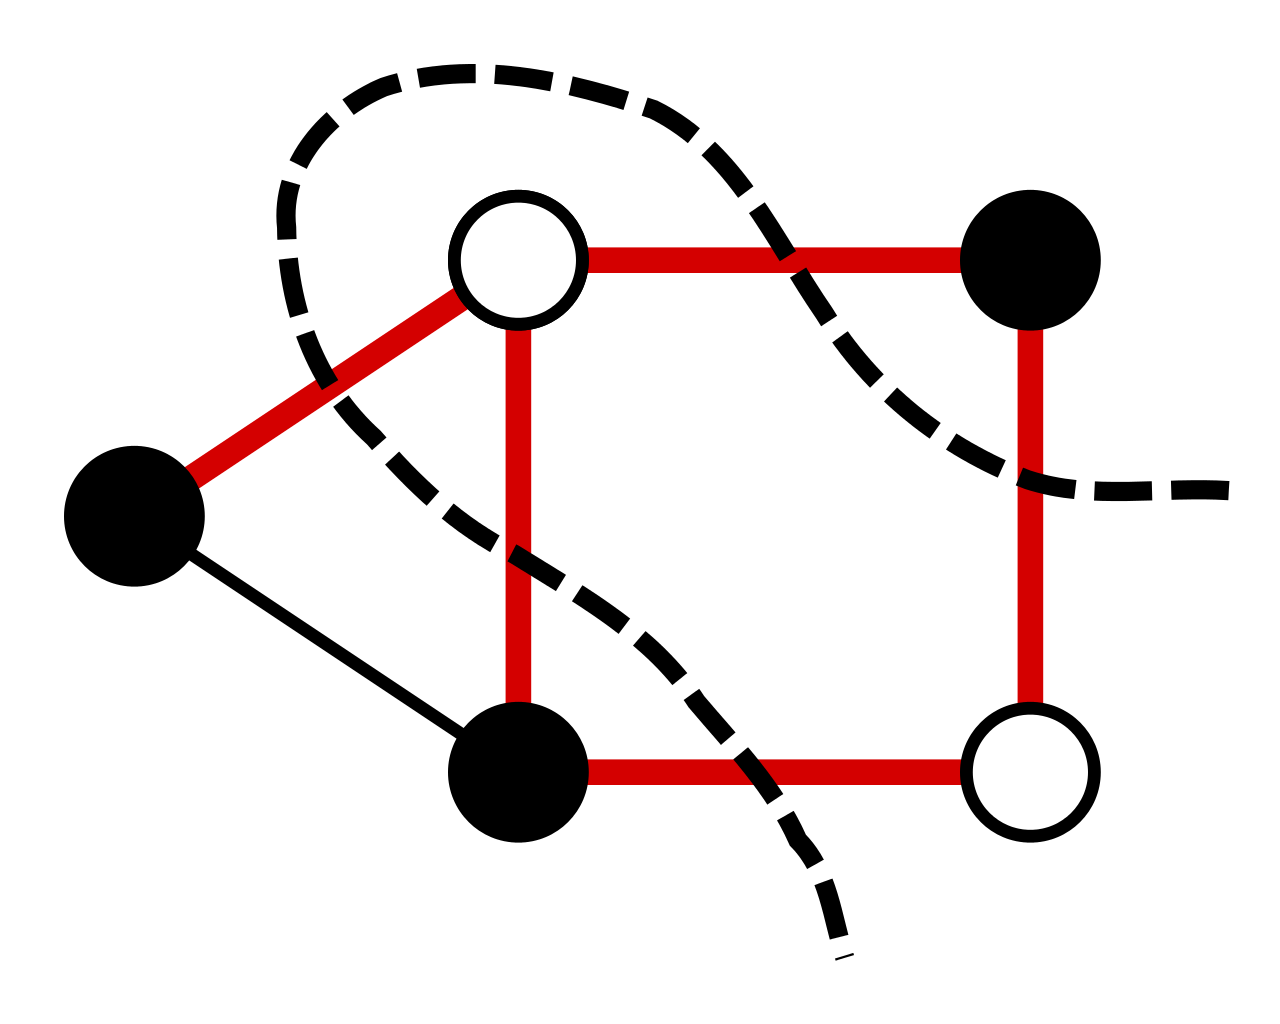
\includegraphics[scale=.2]{1280px-Max-cut.png}
\end{center}
\end{example}


\begin{example}
Si consideramos un grafo completo de 4 vértices, con costo 1 en todas las aristas, el costo de un corte queda determinado por la cantidad de nodos en el corte. Obtenemos los siguientes valores:
$$
\delta(K) = \begin{cases}
0 & \text{ si } \#K = 0, \\
3 & \text{ si } \#K = 1, \\
4 & \text{ si } \#K = 2, \\
3 & \text{ si } \#K = 3, \\
0 & \text{ si } \#K = 4. \\
\end{cases}
$$

Por lo tanto, para obtener el corte de mayor costo tomamos un conjunto $K$ de 2 elementos.
\end{example}



Comenzamos formulando el problema en forma matricial. Queremos calcular el costo de un corte mediante un producto de matrices. Fijamos un corte $K$ y definimos el vector $\xb = (\xb_1, \dots, \xb_n) \in \R^n$ por
$$
x_i = \begin{cases}
1 & \text{ si } v_i \in K \\
-1 &  \text{ si } v_i \notin K
\end{cases}.
$$
De esta forma, $x_i x_j = -1$ si $(i,j) \in \delta(K)$ y $x_i x_j = 1$ si $(i,j) \notin \delta(K)$, y por lo tanto
$$
1 - x_i x_j = \begin{cases}
0 & \text{ si } (i,j) \in \delta(K) \\
2 &  \text{ si } (i,j) \notin \delta(K).
\end{cases}
$$
Obtenemos
$$
w(\delta(K)) = \frac{1}{2}\sum_{i < j}w_{ij}(1-x_i x_j) = \frac{1}{4}\sum_{i \neq j}w_{ij}(1-x_i x_j).
$$
Como además $w_{ii} = 0$ para todo $i$,
$$
w(\delta(K)) = \frac{1}{4}\sum_i \sum_j w_{ij}(1-x_i x_j) = \left(\frac{1}{4}\sum_i \sum_j w_{ij} \right) - \frac{1}{4} x^T W x.
$$

Para poder juntar los últimos dos términos en uno, reescribimos:
$$
\left(\frac{1}{4}\sum_i \sum_j w_{ij} \right) - \frac{1}{4} x^T W x = \left(\frac{1}{4}\sum_i \left(\sum_j w_{ij}\right) x_i x_i \right) - \frac{1}{4} x^T W x.
$$
y definiendo $C \in \R^{n \times n}$ con $c_{ij} = -w_{ij}/4$ para $i \neq j$ y $c_{ii} = \sum_j w_{ij}/4$ para todo $i$ obtenemos
$$
w(\delta(K)) = x^T C x.
$$

Finalmente, como cualquier vector $x \in \{-1, 1\}^n$ define un corte, podemos escribir el problema max-cut como el problema de programación cuadrática entera:
$$
\text{(IQP):} \quad \max x^TCx, x_i \in \{+1, -1\}, i \in N,
$$
o como un problema cuadrático con restricciones cuadráticas no-convexas
$$
\text{(NQCQP):} \quad \max x^TCx, x_i^2 = 1, i \in N.
$$

Ninguna de estas dos formulaciones corresponde a un problema de programación semidefinida. A continuación veremos como relajar las condiciones para obtener un problema SDP.

\subsection{Relajación 1}
Observamos que (NQCQP) es linear en los productos $x_i x_j$ y que estos productos son las coordenadas de la matriz $X = xx^T \in \R^{n \times n}$ de rango 1. Más aún, $X$ es simétrica, $X_{ii} = 1$ para todo $i$ y $X \succeq 0$. Recíprocamente, cualquier matriz de rango 1 con esas propiedades puede escribirse como $xx^T$ para algún vector $x \in \{-1, 1\}^n$. (COMPLETAR DEMOSTRACION: $X = y x^T$, y podemos tomar $y = x$ y como $x_i^2 = 1$ es de la forma buscada.)

Finalmente, como $x^T C x = C \bullet (xx^T)$, obtenemos que (IQP) es equivalente al problema
$$
\max C \bullet X, \quad X_{ii} = 1, i \in N, X \succeq 0, \rank(X) = 1.
$$

Eliminando la restricción del rango, obtenemos el problema SDP
$$
\max C \bullet X, \quad X_{ii} = 1, i \in N, X \succeq 0.
$$

\subsection{Relajación 2}

Observemos que en (IQP) asociamos a cada nodo $v_i$ un valor $x_i \in \{-1, 1\}$, que podemos considerar como un vector unitario de dimensión 1.
Ahora, en cambio, asociamos a cada nodo $v_i$ un vector unitario $p_i \in \R^n$, y consideramos la matrix $\Pb$ con estos vectores como filas. Reemplazamos entonces la función objetivo $C\bullet (xx^T)$ por $C \bullet (PP^T)$ y las restricciones $x_i \in \{+1, -1\}$ por restricciones de los elementos de la diagonal de $PP^T$: $(PP^T)_{ii} = 1$. Como $PP^T$ es  semidefinida positiva, y cualquier matrix semidefinida positiva se puede factorizar de esta forma, vemos que mediante esta construcción obtenemos el mismo problema SDP de antes.
Considerando una matriz $\Pb$ donde todas las filas son de la forma $v$ o $-v$ para un vector unitario $v$, vemos que este problema es efectivamente una relajación del problema (IQP).

\subsection{Relación entre la relajación y el problema original}

Como las formulaciones SDP son relajaciones del problema max-cut, el valor óptimo del problema SDP es una cota superior del valor óptimo del problema original. Pero vamos a ver que podemos usar la solución del problema SDP para obtener un corte razonablemente bueno.

Usamos la segunda relajación, y tomamos $X = PP^T$ una solución óptima de ese problema. Si todas las filas de $\Pb$ fueran $+v$ o $-v$ para un vector $v$, definimos el corte tomando en $K$ todos los nodos para los cuales la fila correspondiente es $+v$.

En la situación general, tomamos un hiperplano que divide a la esfera unitaria en dos mitades y tomamos en $K$ a todos los nodos que quedan en una de estas dos mitades.

Más concretamente, para un vector aleatorio $g$ de norma 1, definimos
$$
K = \{v_i \in V: g^T p_i \ge 0\}.
$$

Esto nos da un corte aleatorio, y podemos calcular la esperanza  del valor del corte (veremos más adelante cómo tomar un vector aleatorio).

La esperanza del valor del corte es
$$
E[w(\delta(K))] = E\left[\sum_{i,j} w_{ij} \one_{(i,j) \in \delta(K)}\right] = \sum_{i,j} w_{ij} \Pr[(i,j) \in \delta(K)].
$$
(observamos que las probabilidades no son independientes, pero no es necesaria independencia para distribuir la esperanza con respecto a la suma).

Calculamos ahora $\Pr[(i,j) \in \delta(K)]$ para $(i,j)$ fijo. Consideramos el plano que pasa por el origen y contiene a los dos vectores $p_i$ y $p_j$. La probabilidad de que un hiperplano separe a los dos vectores es la misma que la probabilidad de que un diámetro en este plano los separe. Esta probabilidad es
$$
GW(K) = \Pr[(i,j) \in \delta(K)] = \frac{\angle(p_i, p_j)}{\pi} = \frac{\arccos(p_i \cdot p_j)}{\pi}.
$$

Por lo tanto, el valor esperado del corte es
$$
E[w(\delta(K))] = \sum_{i,j} w_{ij} \frac{\arccos(p_i \cdot p_j)}{\pi}
$$
y queremos comparar este valor
$$
SDP(K) = \sum_{i,j} w_{ij} \left( \frac{1}{2} - \frac{1}{2} p_i \cdot p_j \right) \ge OPT(K).
$$

Para comparar ambas expresiones término a término, consideramos $\rho = p_i \cdot p_j$, $-1 \le \rho \le 1$ y graficamos las funciones $f_1(\rho) = \frac{\arccos(p_i \cdot p_j)}{\pi}$ y $f_2(\rho)  = \frac{1}{2} - \frac{1}{2} p_i \cdot p_j$.

Calculando la mayor diferencia entre las dos funciones, obtenemos que $f_1(\rho) \ge 0.87584 f_2(rho)$ y por lo tanto:
$$
GW(K) \ge 0.87584 SDP(K),
$$
y esto implica que existe algún corte $K^\star$ tal que $w(\delta(K^\star)) \ge 0.87584$ del valor óptimo del problema SDP.

Para el pentágono con todos los pesos de las aristas iguales a 1, la razón entre el valor óptimo del problema max-cut y la relajación SDP es aproximadamente 0.884, por lo tanto la cota obtenida anteriormente esta cerca de la mejor cota que podemos obtener.

Ejercicio: ¿qué cota podemos obtener en la otra dirección? Es decir, ¿puede ser que el valor obtenido por la relajación SDP coincida con el valor óptimo del problema max-cut? ¿O cuál es la mejor cota que podemos obtener?


\section{Teor\'ia de control en sistemas din\'amicos }

Referencia principal: \cite[Sección 2.2.1]{Blekherman2013}.

Una de las primeras y más importantes aplicaciones de optimización semidefinida es en la teoría de control.
En este caso la programación semidefinida nos permite caracterizar propiedades dinámicas (por ejemplo, estabilidad) en términos de relaciones algebraicas, específicamente como la factibilidad de sistemas de inecuaciones.

Comenzamos con un ejemplo muy sencillo que nos permite darnos una idea de las características de problemas más complicados.

\subsection{Estabilidad de sistemas lineales}

Consideremos una relación de recurrencia lineal,
$$
\xb[k+1] = \Ab \xb[k], \quad \xb[0] = \xb_0,
$$
con $\xb[k] \in \R^n$ para todo $k \in \N_0$ y $\Ab \in \R^{n \times n}$.

Esta relación es un ejemplo simple de un sistema dinámico discreto, el estado $\xb[k]$ evoluciona con el tiempo a partir de un estado inicial $\xb[0]$. El análogo continuo está dado por la ecuación diferencial
$$
\frac{d}{dt}\xb(u) = \Ab\xb(t).
$$
Estos modelos son utilizados para modelar la evolución en el tiempo de cantidades tales como temperatura, tamaño de la población, etc.

Una pregunta natural e importante es el comportamiento en el largo plazo del vector de estados. En particular, queremos determinar condiciones sobre la matriz $\Ab$ que permitan garantizar que el vector de estados se mantenga acotado o converja a 0.

Calculando autovalores y autovectores, sabemos que $\xb[k]$ converge a 0 para todo estado inicial si y solo si el radio espectral $\rho(\Ab) < 1$, es decir si los autovalores $\lambda_i$ de $\Ab$ cumplen $|\lambda_i| < 1$ para todo $1 \le i \le n$. En este caso decimos que el sistema (o la matriz $\Ab$ es estable).

Veremos ahora una forma alternativa de estudiar el problema, que resulta en ciertas ocasiones más conveniente.

Para una matrix $\Pb \in \R^{n \times n}$ positiva semidefinida, definimos la función $V$,
$$
V(\xb[k]) = \xb[k]^T \Pb \xb[T].
$$
Vamos a ver que el sistema es asintóticamente estable si existe $\Pb \succ 0$ tal que $V$ es no-decreciente sobre las trayectorias del sistema. Es decir, si $V(\xb[k+1]) < V(\xb[k])$ para todos los estados $\xb[k]$. Observamos primero que esto es equivalente a la desigualdad de matrices
$$
\Ab^T \Pb \Ab - \Pb \prec 0.
$$
Podemos probar ahora el siguiente resultado.

\begin{theorem}
Dada una matriz $\Ab \in \R^{n \times n}$, las siguientes condiciones son equivalentes:
\begin{enumerate}
\item \label{item:rho} $\rho(\Ab) < 1$
\item \label{item:matrix} Existe una matrix $\Pb \in \R^{n \times n}$ simétrica tal que
$$
\Pb \succ 0, \quad \quad \Ab^T \Pb \Ab - \Pb  \prec 0.
$$
\end{enumerate}
\end{theorem}

\begin{proof}
\ref{item:matrix} $\Rightarrow$ \ref{item:rho}: Dado $\vb \in \C^n$, $\vb \neq 0$, autovector de $\Ab$, $\Ab\vb = \lambda \vb$,
$$
0 > \vb^* (\Ab^T \Pb \Ab - \Pb)\vb = (|\lambda|^2 - 1) \vb^* \Pb \vb,
$$
donde $\vb^* \Pb \vb > 0$ y por lo tanto $|\lambda| < 1$.

\ref{item:rho} $\Rightarrow$ \ref{item:matrix}: Tomamos $\Pb = \sum_{k=0}^{\infty}(\Ab^k)^T \Ab^k$ (como $\rho(\Ab) < 1$, la suma converge). Luego
$$
\Ab^T \Pb \Ab - \Pb = \sum_{k=1}^{\infty} (\Ab^k)^T \Ab^k - \sum_{k=0}^{\infty} (\Ab^k)^T \Ab^k = - \Id \prec 0.
$$
\end{proof}

De esta forma convertimos el problema en un problema de factibilidad de SDP. Observamos que las coordenadas de la matriz $\Ab^T \Pb \Ab - \Pb$ son lineales afines en los coeficientes de $\Pb$, por lo tanto el problema es efectivamente un problema SDP.

\subsection{Diseño de control}
Consideramos ahora una extensión del problema anterior en la que agregamos una señal de control $\ub[k] \in \R^{m}$:
$$
\xb[k+1] = \Ab\xb[k] + \Bb\ub[k], \quad \xb[0] = \xb_0,
$$
con $\Bb \in \R^{n \times m}$. La función del término de control es poder ajustar el comportamiento de $\xb[k]$ para lograr un cierto objetivo. Analizamos en particular el caso en que $\Ab$ no es estable, pero podemos usar un control lineal $\ub[k] = \Kb\xb[k]$ para una matriz fija $\Kb$ (a elegir apropiadamente). En este caso, podemos escribir el sistema de la forma
$$
\xb[k+1] = (\Ab + \Bb\Kb)\xb[k], \quad \xb[0] = \xb_0,
$$
que es equivalente al problema original reemplazando a la matriz $\Ab$ por $\Ab+\Bb\Kb$. Este es un problema de una dificultad mayor al anterior, debido a que los autovalores de $\Ab + \Bb\Kb$ dependen en forma no-lineal de los autovalores de la matriz a calcular $\Kb$. Sin embargo, vamos a ver que podemos resolver este problema por optimización semidefinida usando la caracterización alternativa de Lyapunov.

Utilizando complementos de Schur, podemos reescribir las condiciones
$$
(\Ab+\Bb\Kb)^T \Pb (\Ab + \Bb\Kb) - \Pb \prec 0, \quad \Pb \succ 0,
$$
como
$$
\begin{pmatrix}
\Pb & (\Ab+\Bb\Kb)^T \Pb \\
\Pb(\Ab+\Bb\Kb) & \Pb
\end{pmatrix} \succ 0.
$$
Esta formulación no un problema SDP debido a los términos no-lineales en las entradas de  $\Kb$ y $\Pb$, las matrices a calcular.

Sin embargo, definiendo $\Qb = \Pb^{-1}$ y multiplicando a izquierda y derecha por la matriz
$$
\begin{pmatrix}
\Qb & \cero  \\
\cero & \Qb
\end{pmatrix},
$$
obtenemos la restricción equivalente
$$\begin{aligned}
\begin{pmatrix}
\Qb & \Qb(\Ab+\Bb\Kb)^T  \\
(\Ab + \Bb\Kb)\Qb & \Qb
\end{pmatrix} &=
\begin{pmatrix}
\Qb & \Qb\Ab^T + \Qb\Kb^T\Bb^T  \\
\Ab\Qb + \Bb\Kb\Qb & \Qb
\end{pmatrix} \\
&=
\begin{pmatrix}
\Qb & \Qb\Ab^T + (\Kb\Qb)^T\Bb^T  \\
\Ab\Qb + \Bb\Kb\Qb & \Qb
\end{pmatrix} \succ 0
\end{aligned}
$$
(en la última igualdad utilizamos que $\Qb$ es simétrica).

Si bien parece que no ganamos mucho con esta transformación, observamos ahora que la matriz $\Kb$ siempre aparece multiplicada por $\Qb$ a derecha. Por lo tanto, definiendo $\Yb = \Kb\Qb$, obtenemos la condición
\begin{equation}
\label{eq:QY}
\begin{pmatrix}
\Qb & \Qb\Ab^T + \Yb^T\Bb^T  \\
\Ab\Qb + \Bb\Yb & \Qb
\end{pmatrix}  \succ 0.
\end{equation}

En este caso el problema es lineal en las variables $(\Qb, \Yb)$, y por lo tanto es un problema SDP. Luego de resolver este problema, podemos recuperar la matriz $\Kb$ por la fórmula $\Kb = \Qb^{-1}\Yb$.

Resumimos lo obtenido en el siguiente resultado.

\begin{theorem}
Dadas matrices $\Ab \in \R^{n\times n}$ y $\Bb \in \R^{n \times m}$, existe una matriz $\Kb \in \R^{m \times n}$ tal que $\Ab + \Bb\Kb$ es estable si y solo si el espectrahedro definido por la ecuación \ref{eq:QY} es no vacío, es decir, existen matrices $(\Qb, \Yb)$ tales que se satisface la desigualdad matricial estricta.
\end{theorem}

Concluimos entonces que el problema de control planteado es equivalente a un problema de programación semidefinida.

\subsection{Caso continuo}

Consideramos un sistema dinámico autónomo
$$
\dot{\xb}(t) = \frac{d}{dt}{\xb(t)} =f(\xb(t)),\;\;\;\;\xb(0)=\xb_{0},
$$
y suponemos que se cumple
$$
\dot{\xb}(t)  \in \conv\{\Ab_1, \dots, \Ab_m\} \xb(t),
$$
donde $\conv\{\Ab_1, \dots, \Ab_m\} = \{\alpha_1 \Ab_1 + \dots + \alpha_m \Ab_m : 0 \le \alpha_i \le 1, \sum \alpha_i = 1\}$.

\textbf{Ejemplo.} Si $m = 1$, obtenemos el sistema $\dot{\xb}(t) = \Ab \xb(t)$.

La condición más general nos permite indicar que las derivadas se mueven en ciertos rangos.

Queremos determinar si $\xb(t)$ se mantiene acotada, es decir, si el equilibrio $\xb = \cero$ es estable.

Observamos que $\xb(t)$ se mantiene acotada si y solo si existe $\Pb \succ 0$ tal que
$$
v: \R^n \rightarrow \R, v(\xb) = \xb^T \Pb \xb
$$
se mantiene acotada sobre las trayectorias.

Una condición para asegurar esto es pedir que $v$ sea decreciente sobre las trayectorias.

Estas funciones se conocen como \emph{funciones de Lyapunov}.

Utilizando la regla de derivación de un producto interno para $f, g: \R \rightarrow \R^n$:
$$\frac{d}{dt}(\inner{f(t)}{g(t)}) = \inner{\dot f(t)}{g(t)} + \inner{f(t)}{\dot g(t)},$$
obtenemos que $\xb(t)$ se mantiene acotada si
$$
\dot v(\xb) = \frac{d}{dt}\xb^T \Pb \xb = \dot{\xb}^T \Pb \xb +  {\xb}^T \Pb \dot{\xb} \le 0.
$$

Si $\xb(0)$ es arbitrario y $\dot \xb(0)$ puede estar en cualquier punto del conjunto convexo, necesitamos
$$
\Ab_i^T \Pb + \Pb \Ab_i \preceq 0, \quad \text{ para todo } 1 \le i \le m.
$$

\subsection {Problema SDP}

Las restricciones obtenidas corresponden a un problema SDP.

Si buscamos $\Pb \succ 0$ bien condicionada, definimos el siguiente problema SDP:
\begin{alignat*}{2}
  & \text{minimizar: } & & \eta \\
   & \text{sujeto a: } & \quad & \Ab_i^T \Pb + \Pb \Ab_i \preceq 0, \quad \text{ para todo } 1 \le i \le m \\
   &&& \eta \Ib \succeq \Pb \succeq \Ib
\end{alignat*}
donde las variables del problema son $\eta$ y las entradas de $\Pb$.




\section{Conjuntos estables en grafos}

Referencia principal: \cite[Sección 2.2.3]{Blekherman2013}.

El c\'odigo gen\'etico est\'a compuesto por secuencias de bases, que podemos representar por las letras A, C, D y G. En algunos problemas de diseño de código genético es importante evitar las repeticiones en el código.

Si pensamos a distintas secuencias de c\'odigo gen\'etico como nodos en un grafo, y unimos con aristas los pares de secuencias que presentan alguna repetición, el problema de evitar repeticiones se traduce en seleccionar la mayor cantidad de nodos tales que no haya dos nodos conectados entre s\'i.

En la teor\'ia de grafos, esto se traduce como un subgrafo estable.

Dado un grafo no dirigido $G = (V, E)$, un conjunto estable (o conjunto independiente) es un subconjunto de $S \subset V$ tal que el grafo inducido por $S$ no tiene ninguna arista, es decir, no hay dos vértices de $S$ conectados por una arista en $E$.

El número de estabilidad de un grafo, que notamos $\alpha(G)$, es el cardinal del mayor conjunto estable. Calcular el número de estabilidad de un grafo es en general NP-hard. Veremos ahora como obtener una relajación SDP que nos permite dar una cota superior de $\alpha(G)$.

Dado un conjunto $S \subset V$, definimos el vector indicador $\chi(S)$,
$$
\chi(S) = \begin{cases}
1 &\text{ si } v_i \in S \\
0 &\text{ si no}
\end{cases}.
$$

Observamos que la matriz $\Yb = \chi(S) \chi(S)^T$ cumple las siguientes propiedades:
\begin{itemize}
\item $\Yb \succeq 0$.
\item $y_{ij} = 1$ si y solo si $v_i \in S$ y $v_j \in S$. Por lo tanto, $\sum_{i,j} y_{ij} = |S|^2$.
\item En particular $y_{ii} = 1$ si y solo si $v_i \in S$. Por lo tanto, $\Tr(\Yb) = \sum_{i} y_{ii} = |S|$.
\end{itemize}

Tomando $X = \frac{1}{|S|} \Yb$, vemos que $\sum_{i,j} \xb_{ij} = |S|$ y $\Tr(\Xb) = 1$. Luego $\Xb$ es una solución factible del siguiente problema de programación semidefinida:
\begin{alignat*}{2}
  & \text{maximizar: } & & \Tr JX \\
   & \text{sujeto a: } & \quad & \Tr X = 1 \\
   & & & X_{ij} = 0 \text{ para } (i,j) \in E, \\
   & & & X \succeq 0,
\end{alignat*}
donde $J \in \R^{n \times n}$ es la matriz con 1 en todas las coordenadas.

Para un grafo $G$ definimos la función theta de Lovász $\vartheta(G)$ como el valor óptima el problema SDP dado.
Como la matriz $X$ construida a partir de un subconjunto $S \subset V$ es una solución factible, obtenemos que
$$ \alpha(G) \le \vartheta(G),$$
es decir $\vartheta(G)$ es una cota superior de $\alpha(G)$, el número de estabilidad de $G$.

\section{Distancia euclídea}

Consideramos un grafo $G = (N, E)$ con nodos $N = \{1, \dots, n\}$, aristas $E \subset N \times N$, y pesos no negativos $D = \{d_{ij}\} \in \R_+^E$, que representan distancias entre los nodos.

Decimos que $(G, D)$ es $k$-realizable si podemos ubicar los nodos de $G$ en puntos $\vb_1, \dots, \vb_n \in \R^k$ de forma tal que las distancias euclídeas entre los nodos respeten las longitudes dadas:
$$
\exists \vb_1, \dots, \vb_n \in \R^k:  \| \vb_i - \vb_j \| = d_{ij} \quad \forall \{i, j\} \in E.
$$

Decimos que $(G, D)$ es realizable (a secas) si existe $k$ tal que $(G, D)$ es $k$-realizable.

\subsection{Grafo completo}

Para el caso de un grafo completo tenemos la siguiente caracterización.

\begin{theorem}
Sea $G = K_n$ un grafo completo, con pesos $D$, y sea $\Ab \in \Sym^{n}$ la matriz
{\small
$$
\Ab = \begin{pmatrix}
0 & d_{21}^2 & d_{31}^2 & \dots & d_{n1}^2 \\
d_{21}^2 & 0 & d_{32}^2 & \dots & d_{n2}^2 \\
\vdots & \vdots & \vdots & \ddots & \vdots \\
d_{n1}^2 & d_{n2}^2 & d_{n3}^2 & \dots & 0
\end{pmatrix}.
$$}
\vspace{-0.5cm}

El grafo $G$ es realizable si y solo si $\Ab$ es semidefinida negativa en el espacio ortogonal al vector $\eb = (1, 1, \dots, 1)$. Es decir, si
$$
\yb^T \Ab \yb \le 0 \quad \text{ para todo } \yb \in \R^n \text{ tal que } \sum_{i=1}^n y_i = 0.
$$
\end{theorem}

\begin{proof}
Demostramos solo $\Rightarrow$.
Suponemos que para algún $k \ge 1$ existen vectores $\vb_i \in \R^k$, $1 \le i \le n$, tales que $d_{ij} = \|\vb_i - \vb_j\|$. Consideramos ahora la matriz $\Xb$ de productos internos
$$
\Xb = \begin{pmatrix}
\innerl{\vb_1}{\vb_1} & \innerl{\vb_1}{\vb_2} & \dots & \innerl{\vb_1}{\vb_n} \\
\innerl{\vb_2}{\vb_1} & \innerl{\vb_2}{\vb_2} & \dots & \innerl{\vb_2}{\vb_n} \\
\vdots & \vdots & \ddots & \vdots \\
\innerl{\vb_n}{\vb_1} & \innerl{\vb_n}{\vb_2} & \dots & \innerl{\vb_n}{\vb_n}
\end{pmatrix} = (\vb_1 \dots \vb_n)^T (\vb_1 \dots \vb_n),
$$
que es semidefinida positiva. Como $a_{ij} = \| \vb_i - \vb_j\|^2 = \innerl{\vb_i}{\vb_i} + \innerl{\vb_j}{\vb_j} - 2 \innerl{\vb_i}{\vb_j}$, tenemos
$$
\Ab = \inner{\diag(\Xb)}{\eb^T} + \inner{\eb}{\diag(\Xb)} - 2 \Xb.
$$

Por lo tanto, para $\yb \perp \eb$, $\yb^T \Ab \yb = -2 \yb^T \Xb \yb \le 0$.

\end{proof}

\subsection{Grafos no completos}

En general, para grafos no completos determinar si el grafo es realizable equivale a buscar una solución factible de un problema SDP.

\begin{theorem}
Un grafo con pesos $(G, D)$ es realizable si y solo si el siguiente problema SDP tiene solución
\begin{alignat*}{2}
  & \text{existe: } & & \Xb \in \Sym^n \\
   & \text{sujeto a: } & \quad & x_{ii} + x_{jj} - 2 x_{ij} = d_{ij}^2 \quad \forall \{i, j\} \in E, \\
   &&& \Xb  \succeq 0
\end{alignat*}

Más aún, $(G, D)$ es $k$-realizable si existe una solución $\Xb$ de rango a lo sumo $k$.
\end{theorem}

\begin{proof}
Si $\vb_1, \dots, \vb_n \in \R^k$ es una realización de $(G, D)$, entonces la matriz de Gram
$$
\Xb = (\innerl{\vb_i}{\vb_j}) = (\vb_1 \dots \vb_n)^T (\vb_1 \dots \vb_n)
$$
es una solución del problema, de rango a lo sumo $k$.

Recíprocamente, si $\Xb$ es una solución del problema, podemos encontrar una descomposición
$$
\Xb = \Vb^T \Vb, \quad \Vb \in \R^{k \times n}
$$
y tomamos como $\vb_i$ las columnas de $\Vb$.
\end{proof}

\subsection{Grafos completos revisitados}

Utilizando el último teorema obtenemos otra caracterización para grafos completos.

\begin{theorem}
Sea $G = K_n$ grafo completo, con pesos $D$, y sea $\Xb \in \Sym^{n-1}$ la matriz definida por
\begin{align*}
x_{ii} &= d_{in}^2, \quad \forall 1 \le i \le n-1 \\
x_{ij} &= \frac{d_{in}^2 + d_{jn}^2 - d_{ij}^2}{2}, \quad \forall 1 \le i \neq j \le n-1.
\end{align*}

Entonces $K_n$ es $k$-realizable si y solo si $\Xb \succeq 0$ y $\rank \Xb \le k$.
\end{theorem}

\textbf{Idea de la demostración.} Si el problema SDP tiene solución factible, mediante una traslación, podemos suponer $\vb_n = \cero$.

\subsection{El problema de la partición}

Como vimos, determinar si un grafo $(G, D)$ es realizable, puede resolverse eficientemente por optimización semi-definida.
Sin embargo, determinar si es $k$-realizable para un $k$ dado es un problema mucho más difícil.

Veremos un caso simple en el que el problema es NP-completo.

Consideramos el siguiente problema para el cual se sabe que es NP-completo.

\begin{problem}[El problema de la partición]
Dada una secuencia de números naturales $a_1, \dots, a_n \in \N$, determinar si los números pueden separarse en dos conjuntos con la misma suma. Es decir, si existe $\bm{\epsilon} \in \{\pm 1\}^n$ tal que
$$
\epsilon_1 a_1 + \dots + \epsilon_n a_n = 0.
$$
\end{problem}

\subsection{Grafo ciclo}

Un grafo $(G, E)$ se llama ciclo o cíclico si las aristas forma un ciclo de longitud $n$. Es decir, podemos suponer que las aristas son $(i, i+1)$ para $1 \le i \le n-1$ y $(n, 1)$.

\begin{theorem}
Dado un grafo ciclo $(G, E)$ con pesos naturales $d \in \N^E$, decidir si $(G,D)$ es $1$-realizable es un problema NP-completo.
\end{theorem}

\begin{proof}
Para una instancia $a_1, \dots, a_n \in \N$ del problema de la partición, consideramos el grafo ciclo $(G,E)$ con pesos $d_{i(i+1)} = a_i$.

Si $(G,D)$ es $1$-realizable, con $v_i \in \R$, definimos
$$
\begin{cases}
\epsilon_i = 1 & \text{ si } v_{i+1} > v_i \\
\epsilon_i = -1 & \text{ si } v_{i+1} < v_i
\end{cases}
$$
y obtenemos una partición de los $a_i$.
\end{proof}

\subsection{Rango 1 y rango 2}

Puede demostrarse la siguiente propiedad:

\begin{center}
Un grafo ciclo es realizable si y solo si es $2$-realizable.
\end{center}

\begin{ejercicio} Ver geométricamente que puedo llevar una realización 3D de un grafo ciclo a una realización 2D.
\end{ejercicio}

Concluimos que es posible contestar eficientemente si un grafo ciclo es realizable en un plano o una recta, pero determinar en cuál de los dos es un problema NP-completo.

\section{Minimización de rango}

Como vimos, un problema interesante en optimización es el problema de la minimización de rango, que podemos plantear en la forma
\begin{alignat*}{2}
  & \text{minimizar: } & & \rank \Xb  \\
   & \text{sujeto a: } & \quad & \Xb  \in \mathcal{C},
\end{alignat*}
donde la matriz $\Xb \in \R^{m \times n}$ es la variable de decisión, y $\mathcal{C}$ es un conjunto convexo. Como la función a optimizar tiene valores enteros, este problema en general no es un problema convexo. En el ejemplo anterior vimos que en general es un problema NP-completo.

\subsection{Ejemplo - El problema de Netflix}

\begin{itemize}
\item Algunos usuarios califican algunas de las películas que vieron.
\item Los puntajes son números enteros entre 1 y 5.
\item Queremos predecir los puntajes para cada par usuario / película.
\item Es decir, queremos completar una matriz incompleta como la de la figura.
\end{itemize}
\begin{center}
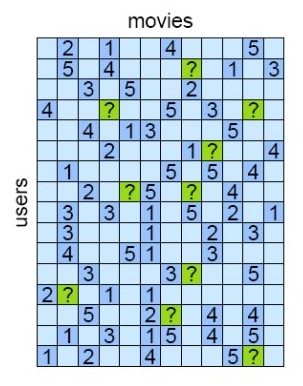
\includegraphics[scale=.6]{rank_netflix.jpg}
\end{center}

Si pensamos que hay unos pocos perfiles de usuarios arquetípicos (amante de las películas de terror, románticas, comedias, etc.) y cada usuario es una combinación lineal de esos perfiles, podemos factorizar la matriz:

\begin{center}
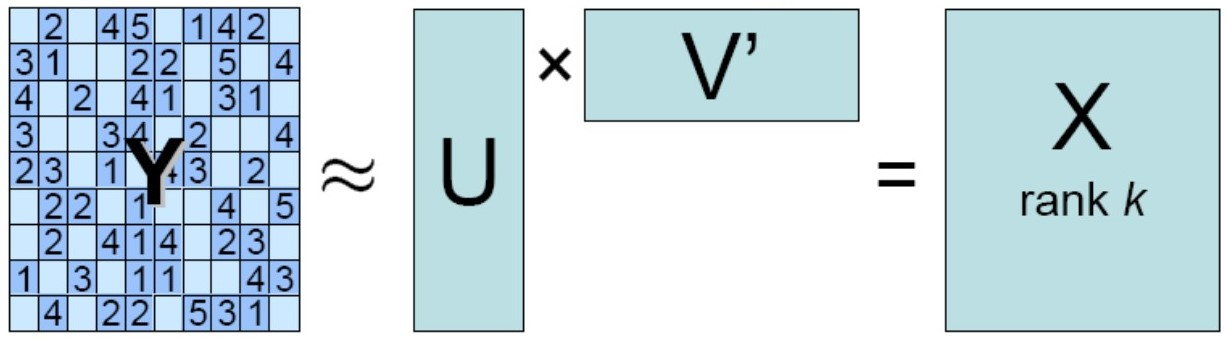
\includegraphics[scale=.4]{rank_factorization.jpg}
\end{center}

\subsection{Rango y valores singulares}

\begin{itemize}
\item Para una matriz $\Ab \in \Rnn$ cuadrada, el rango de $\Ab$ es igual a la cantidad de autovalores no-nulos.
\item Para una matriz $\Ab \in \R^{m \times n}$, el rango de $\Ab$ es igual a la cantidad de valores singulares no-nulos.
\end{itemize}

\textbf{Heurística}
\begin{itemize}
\item Como no podemos minimizar el rango eficientemente, minimizamos la suma de los valores singulares.
\item Para $\Ab \succeq 0$, la suma de los valores singulares es igual a $\Tr(\Ab)$, que es una función lineal en los coeficientes de $\Ab$.
\end{itemize}

\subsection{Norma nuclear}

\begin{minipage}[c]{0.7\textwidth}
En $\R^{m \times n}$ definimos la norma nuclear
$$
\| \Xb \|_* = \sum_{i=1}^{\min\{m, n\}} \sigma_i.
$$

Como los valores singulares son todos no-negativos,
$$
\| \Xb \|_* = \| \bm{\sigma} \|_1.
$$

Comparando las curvas de nivel distintas normas, vemos que minimizando la norma-1 obtenemos en general vectores esparsos con gran cantidad de 0's. Por este motivo es una buena elección para obtener matrices de rango bajo.
\end{minipage}
\begin{minipage}[c]{0.25\textwidth}
\begin{center}
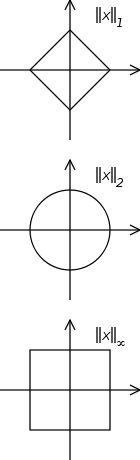
\includegraphics[scale=.4]{140px-Vector_norms.png}
\end{center}
\end{minipage}

Para analizar las propiedades de la norma nuclear, recordemos las siguientes propiedades:
\begin{itemize}
\item Para $\Ab, \Bb \in \R^{m \times n}$,
$$\innerTrace{\Ab}{\Bb} = \tr(\Ab^T \Bb)= \tr(\Ab \Bb^T)$$
es un producto interno en $\R^{n \times n}$, que define la norma
$$\|\Ab\|_F = \sqrt{\innerTrace{\Ab}{\Ab}} = \sqrt{\Tr(\Ab \Ab^T)}.$$

Si $\Xb = \Ab \Ab^T$, $\Tr(\Xb) = \|\Ab\|_F^2$.
\item Desigualdad de Cauchy-Schwarz: $|\langle \ub, \vb \rangle| \le \|\ub\| \|\vb\|$
\item Desigualdad MA-MG: $\|\ub\| \|\vb\| \le \frac{1}{2}(\|\ub\|^2 + \|\vb\|^2)$
\end{itemize}

\begin{lemma}
Para $\Xb \in \R^{n \times n}$,
$$
\|\Xb\|_* = \min_{\Xb = \Ub \Vb^T} \|\Ub\|_{F} \|\Vb\|_{F} = \min_{\Xb = \Ub \Vb^T} \frac{1}{2}(\|\Ub\|^2 + \|\Vb\|^2).
 $$
\end{lemma}

{\small Este y los siguientes resultados valen también para $\Xb$ rectangular.}

\begin{proof} Tomamos una descomposición SVD de $\Xb$,
$$\Xb = \Pb \Sb \Qb^T,$$
con $\Pb \in \R^{n \times n}$ unitaria, $\Sb \in \R^{n \times n}$ diagonal, con los valores singulares $\sigma_1 \ge \sigma_2 \ge \dots \ge \sigma_n \ge 0$ en la diagonal y $\Qb \in \R^{n \times n}$ unitaria.

Si $\Xb = \Ub \Vb^T$, con $\Ub \in \R^{n \times k}$, $\Vb \in \R^{n \times k}$, entonces
\begin{align*}
\|\Xb\|_* &= \tr(\Sb) = \tr(\Pb^T \Ub \Vb^T \Qb) \\
&= \innerTrace{\Pb^T \Ub}{\Qb^T \Vb} \le \|\Pb^T \Ub\|_F\|\Qb^T \Vb\|_F \\
&=  \|\Ub\|_F\|\Vb\|_F \le \frac{1}{2}(\|\Ub\|_F + \|\Vb\|_F),
\end{align*}
donde $\Pb^T\Ub, \Qb^T\Vb \in \R^{n \times k}$.

Tomando $\Ub = \Pb \Sb^{\frac12}$ y $\Vb = \Qb \Sb^{\frac12}$, alcanzamos el mínimo.
\end{proof}

Utilizando el lema, obtenemos una caracterización de la norma nuclear por un problema SDP.

\begin{lemma}
Para cualquier matriz $\Xb \in \R^{n \times n}$ y $t \in \R$, $\|\Xb\|_* \le t$ si y solo si existen $\Ab \in \R^{n \times n}$ y $\Bb \in \R^{n \times n}$ tales que
$$
\begin{pmatrix} \Ab & \Xb \\ \Xb^T & \Bb \end{pmatrix} \succeq 0 \quad \text{ y } \quad \tr(\Ab) + \tr(\Bb) \le 2t.
$$
\end{lemma}

\begin{proof}
Si $\begin{pmatrix} \Ab & \Xb \\ \Xb^T & \Bb \end{pmatrix} \succeq 0$, podemos factorizarla
$$
\begin{pmatrix} \Ab & \Xb \\ \Xb^T & \Bb \end{pmatrix} = \begin{pmatrix} \Ub \\ \Vb \end{pmatrix}
\begin{pmatrix} \Ub^T & \Vb^T \end{pmatrix},
$$
con $\Ub \in \R^{n \times (n+n)}$ y $\Vb \in \R^{n \times (n+n)}$.

Tenemos $\Ab = \Ub \Ub^T$,  $\Bb = \Vb \Vb^T$ y $\Xb = \Ub \Vb^T$.

Por lo tanto, $\|\Ub\|_F^2 + \|\Vb\|_F^2 = \tr \Ab + \tr \Bb \le 2t$, y obtenemos
$$\|\Xb\|_* \le \frac{1}{2}(\|\Ub\|^2 + \|\Vb\|^2) \le t.$$

Recíprocamente, si $\|\Xb\|_* \le t$,
y $\Xb = \Pb \Sb \Qb^T$ es una descomposición SVD, tomando
$\Ub = \Pb \Sb^{\frac12}$ y $\Vb^T = \Sb^{\frac12} \Qb^T$, obtenemos
$$
\Zb = \begin{pmatrix} \Ub \\ \Vb \end{pmatrix}
\begin{pmatrix} \Ub^T & \Vb^T \end{pmatrix} = \begin{pmatrix} \Ub\Ub^T & \Xb \\ \Xb^T & \Vb \Vb^T \end{pmatrix} \succeq 0$$
y $\tr(\Zb) = \tr(\Ub\Ub^T) + \tr(\Vb\Vb^T) \le 2t$.

\end{proof}

\subsection{Norma nuclear como problema SDP}

Extendiendo los resultados anteriores a matrices rectangulares (ejercicio), obtenemos que la norma nuclear $\|\Xb\|_*$, $\Xb \in \R^{m \times n}$, se corresponde con el valor óptimo del problema SDP
\begin{alignat*}{2}
  & \text{minimizar: } & & \frac{1}{2}\Tr \begin{pmatrix} \Ab & \Xb \\ \Xb^T & \Bb \end{pmatrix} \\
   & \text{sujeto a: } & \quad & \begin{pmatrix} \Ab & \Xb \\ \Xb^T & \Bb \end{pmatrix}   \succeq 0
\end{alignat*}
para matrices $\Ab \in \R^{m \times m}$, $\Bb \in \R^{n \times n}$.

Para el problema de Netflix, obtenemos que el problema de completar una matriz $\Mb \in \R^{m \times n}$ para la cual solo se conocen algunas casillas $m_{ij}$, $(i,j) \in I$ de forma tal que la norma nuclear sea mínima es equivalente a resolver el problema
\begin{alignat*}{2}
  & \text{minimizar: } & & \frac{1}{2}\Tr \begin{pmatrix} \Ab & \Xb \\ \Xb^T & \Bb \end{pmatrix} \\
   & \text{sujeto a: } & \quad & x_{ij} = m_{ij}, (i, j) \in I, \\
   &&& \begin{pmatrix} \Ab & \Xb \\ \Xb^T & \Bb \end{pmatrix}   \succeq 0
\end{alignat*}
para matrices $\Xb \in \R^{m \times n}$, $\Ab \in \R^{m \times m}$, $\Bb \in \R^{n \times n}$.

Más generalmente, podemos reemplazar la restricción $x_{ij} = m_{ij}, (i, j) \in I$, por $\Xb  \in \mathcal{C}$, para $\mathcal{C}$ un conjunto convexo (definido por restricciones lineales).

\subsection{Ejemplo: sumas de cuadrados}

Determinar si un polinomio $f \in \R[x_1, x_2, x_3]$ homogéneo de grado 4 es suma de cuadrados, es equivalente a determinar si existe una matrix $\Ab$ semidefinida positiva tal que
$$
f = \vb^T  \Ab \vb,
$$
para $\vb = \begin{pmatrix} x_1^2, x_2^2, x_3^2, x_1 x_2, x_1 x_3, x_2 x_3 \end{pmatrix}$.

La escritura como suma de cuadrados se puede obtener factorizando $\Ab = \Xb^T \Xb$ y el rango de $\Ab$ nos dice la cantidad de polinomios linealmente independientes en la descomposición.

Si queremos estudiar el problema de hallar la menor cantidad de polinomios que aparecen en una descomposición, debemos minimizar el rango de la matriz $\Ab$.


\subsection{Norma nuclear de matrices simétricas}

Si trabajamos con matrices simétricas, minimizar la norma nuclear equivale a resolver el problema SDP:

\begin{alignat*}{2}
  & \text{minimizar: } & & \Tr \Xb \\
   & \text{sujeto a: } & \quad & \Xb  \in \mathcal{C}, \\
   &&& \Xb \succeq 0.
\end{alignat*}

\chapter{Polinomios positivos y sumas de cuadrados}
%\noindent Referencia principal: \cite[Capítulo 3]{Lasserre2010}.

\section{Introducci\'on}


Notamos $\R[\xb] = \R[x_1, \dots, x_n]$ al anillo de polinomios sobre $\R$ en $n$ variables.

Dado un polinomio $p(\xb) \in \R[\xb]$, decimos que
\begin{itemize}
\item $p$ es \emph{positivo} ($p \ge 0$) si $p(\xb) \ge 0$ para todo $\xb \in \R^n$ (y \emph{estrictamente positivo} si $p > 0$ para todo $\xb \in \R^n$).
\item $p$ es una \emph{suma de cuadrados} (SOS) si existen $q_1, \dots, q_s \in \R[\xb]$ tales que
$$
p = q_1^2 + \dots + q_s^2.
$$
\end{itemize}

\begin{prop}
Si $p$ es SOS entonces $p \ge 0$.
\end{prop}

\begin{problem}
Dado un polinomio $p(\xb) \in \R[\xb]$, determinar si se puede escribir como suma de cuadrados (SOS) $p = p_1^2 + \dots + p_s^2$ y construir la descomposici\'on (aproximada o exacta).
\end{problem}

Algunas aplicaciones de sumas de cuadrados son:
\begin{itemize}
\item certificados de positividad,
\item La ecuación $p(\xb) + 1 = 0$ no tiene soluciones reales si $p$ es una suma de cuadrados,
\item Dado un polinomio $p$, si queremos hallar el mínimo de $p$ en $S = \R^n$ o en una regi\'on $S = \{ \xb \in \R^n : g(\xb) \ge 0\}$, para polinomios $\{g_1, \dots, g_s\}$, tenemos
\[
\min\{f(x) : \xb \in S\} = \sup\{a \in \R | f - a \ge 0 \text{ en } S\}.
\]
\end{itemize}


\section{Sumas de cuadrados en una variable}

\begin{proposition}
Si $p \in \R[x]$ (polinomios en una variable) entonces
$$
p \text{ es suma de cuadrados } \iff p \text{ es positivo}
$$
\end{proposition}

\begin{proof}
Tomamos $p \ge 0$. Por el teorema fundamental del \'algebra, podemos factorizar
\[
p(x) = \prod_{i=1}^r (x-a_i) \prod_{j=1}^t (x-b_j)(x - \bar b_j),
\]
donde $a_i \in \R$ son las raíces reales y $b_j, \bar b_j \in \C \smallsetminus \R$ son las raíces complejas conjugadas.

Si la multiplicidad de alguna raíz real $a$ es impar, entonces $p$ atraviesa transversalmente al eje $X$ en $a$ y por lo tanto no puede ser $p \ge 0$.

Por lo tanto, todas las raíces reales aparecen con multiplicidad par y podemos factorizar
\[
p(x) = \prod_{i=1}^s (x-a_i)^{2k_i} \prod_{j=1}^t (x-b_j)(x - \bar b_j).
\]

Para las raíces complejas tenemos
\begin{align*}
(x-b_j)(x - \bar b_j) &= (x - (\alpha_i + I \beta_i  ))(x - (\alpha_i - I  \beta_i )) \\
&= ((x - \alpha_i) - I\beta_i  ))((x - \alpha_i) + I \beta_i  )) \\
&= (x - \alpha_i)^2 + \beta_i^2,
\end{align*}
que es una suma de cuadrados.

Concluimos que $p(x)$ es un producto de sumas de cuadrados, y por lo tanto, distribuyendo los productos, $p(x)$ es una suma de cuadrados.

Más aún, utilizando la identidad
\[
(a^2+b^2)(c^2+d^2) = (ac+bd)^2 + (ad-bc)^2
\]
podemos escribir a cualquier polinomio $p(x) \ge 0$ como suma de 2 cuadrados.

\end{proof}


\section{Sumas de cuadrados en varias variables}

\begin{prop}
El polinomio
\[
f(x, y) = x^4y^2 + x^2y^4 - 3x^2y^2+1
 \]
 es no-negativo en $\R^2$ pero no puede escribirse como suma de cuadrados. (Motzkin, 1967)
\end{prop}

\begin{proof}
Veamos primero $f \ge 0$. Por la desigualdad aritmética-geométrica,
$$
\frac{x^4y^2 + x^2y^4 + 1}{3} \ge \sqrt[3]{(x^4y^2)(x^2y^4) 1} = \sqrt[3]{x^6y^6} = x^2y^2,
$$
y despejando obtenemos $x^4y^2 + x^2y^4 - 3x^2y^2+1 \ge 0$

Para ver que el polinomio de Motzkin no es una suma de cuadrados, 
escribimos $f = p_1^2 + \dots + p_s^2$, $p_i \in \R[x, y, z_1, ...,z_m]$. Vamos obteniendo condiciones sobre los posibles polinomios que pueden aparecer en la descomposición.

\begin{enumerate}
\item Podemos evaluar $z_i=0$ para todo $i$ y obtenemos una descomposición en $\R[x, y]$.
\item Si tomamos un monomio $m$ en los $p_i$ con el mayor grado $d$ en $x$, el monomio $m^2$ no se va a cancelar en la suma, y por lo tanto debe ser un monomio de $f$.
\item Por lo tanto, debe ser $d \le 2$.
\item Luego, siguiendo el mismo razonamiento, no puede aparecer $x^2y^2$ en ningún $p_i$.
\item Luego, tampoco pueden aparecer $x^2$ ni $y^2$ en ningún $p_i$.
\item Finalmente, no puede aparecer $x$ ni $y$ en ningún $p_i$.
\item Concluimos que los polinomios $p_i$ son de la forma
$$
a x^2y + b x y^2 + c xy + d,
$$
con $a, b, c, d \in \R$.
\item Al elevar al cuadrado un polinomio de esta forma, el coeficiente de $x^2y^2$ es siempre no-negativo. ¡Absurdo!
\end{enumerate}

\end{proof}

%------------------------------------------------------------------

Podemos extender el razonamiento anterior a casos más generales. Comenzamos realizando algunas definiciones.

\begin{definition}
Dado un vector $\ab \in \N_0^n$, $\ab = (a_1, \dots, a_n)$, definimos el monomio $m = \xb^{\ab}$ como
$$
\xb^{\ab} = x_1^{a_1} x_2^{a_2} \cdots x_n^{a_n},
$$
y análogamente, para un monomio $m$ de esa forma, llamamos a $\ab = (a_1, \dots, a_n) \in \R^n$ su \emph{vector de exponentes}.
\end{definition}

\begin{definition}
Dado un polinomio $p \in \K[\xb]$, definimos el \emph{soporte} de $p$, $\supp(p)$, como el conjunto de todos los vectores de exponentes de los monomios que aparecen en $p$.

Definimos  su \emph{polítopo de Newton} $\mathcal{N}(p)$ como la cápsula convexa de los vectores de exponentes de los monomios que aparecen en $p$,
$$
\mathcal{N}(p) = \conv(\supp(p)).
$$
\end{definition}

Por ejemplo, si $p = x_1 x_2^2 + x_2^2 + x_1 x_2 x_3$ entonces
$$
\mathcal{N}(p) = \conv{(\{(1,2,0), (0,2,0), (1,1,1)\})},
$$
que es un triángulo en $\R^3$.

Utilizando el polítopo de Newton podemos obtener información sobre los monomios que pueden aparecer en una suma de cuadrados.

\begin{theorem}
Si $p = \sum_{i = 1}^s q_i^2$ es una suma de cuadrados, entonces
$$
\mathcal{N}(q_i) \subset \frac{1}{2}\mathcal{N}(p).
$$
\end{theorem}

\begin{proof}
Consideramos la cápsula convexa de la unión de todos los polítopos de Newton de los $q_i$, $1 \le i \le s$,
$$
K = \conv(\cup_{i=1}^s\mathcal{N}(q_i)).
$$

Recordamos que un polítopo está generado por las combinaciones convexas de sus vértices.

Tomamos un \emph{vértice} $\vb$ de $K$ y suponemos por contradicción que $2\vb \not\in \supp(p)$.

Si $\alpha \xb^{\vb}$ aparece en $q_i$, entonces $\alpha^2 \xb^{2\vb}$ aparece en $q_i^2$ con coeficiente $\alpha^2 > 0$. Para que estos términos se cancelen, debe aparecer también $\xb^{2\vb}$ como producto cruzado de términos de algunos $q_i$.

Es decir, existen $\ub, \wb \in K$ tales que $2\vb = \ub+\wb$.

Pero luego, $\vb = \frac{\ub+\wb}{2} \in K$ no es un vértice, lo que contradice la hipótesis.

Concluimos que para cualquier vértice $\vb$ de $K$, $2\vb \in \supp(p) \subset \mathcal{N}(p)$.

Como $2K$ es un polítopo, es la cápsula convexa del conjunto de todos sus vértices.

Como todos los vértices de $2K$ están contenidos en el conjunto convexo $\mathcal{N}(p)$, obtenemos $2K \subset \mathcal{N}(p)$.

Por lo tanto, $2 \mathcal{N}(q_i) \subset \mathcal{N}(p)$ para todo $1 \le i \le n$.

\end{proof}

\textbf{Motzkin revisitado}

Utilizando este resultado podemos simplificar la demostración de que el polinomio de Motzkin $f(x, y) = x^4y^2 + x^2y^4 - 3x^2y^2+1$ no es una suma de cuadrados.

A la izquierda representamos el polítopo de Newton $\mathcal{N}(f)$ y a la derecha $\frac{1}{2}\mathcal{N}(f)$.

\begin{figure}
    \centering
    \begin{minipage}{0.45\textwidth}
        \centering
        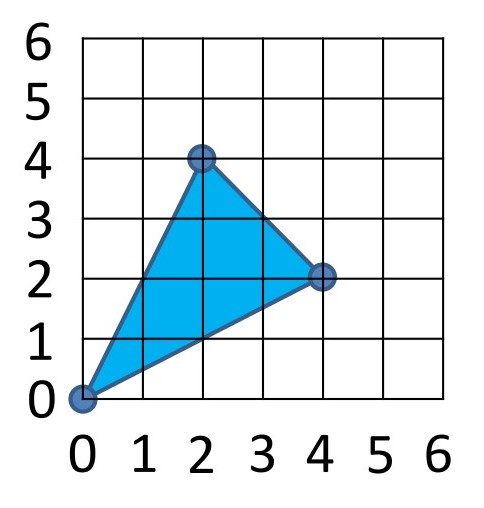
\includegraphics[width=0.5\textwidth]{sos_motzkinHull-2.jpg} % first figure itself
        %\caption{first figure}
    \end{minipage}\hfill
    \begin{minipage}{0.45\textwidth}
        \centering
        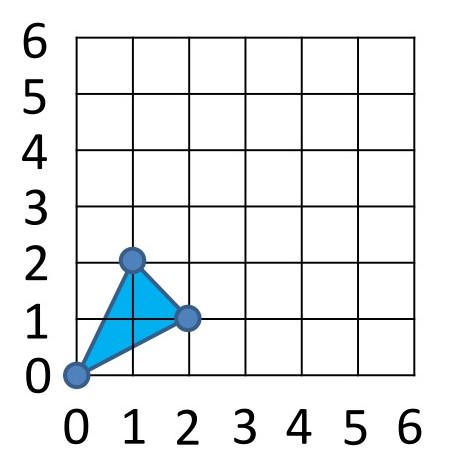
\includegraphics[width=0.5\textwidth]{sos_motzkinHull-3.jpg} % second figure itself
        %\caption{second figure}
    \end{minipage}
\end{figure}

Concluimos inmediatamente que $f = \sum_{i=1}^s q_i$, los $q_i$ son de la forma
$$
q_i(x, y) = a x^2y + b x y^2 + c xy + d.
$$


\textbf{Grado de un polinomio}

Definimos el grado de un monomio $x_1^{a_1} \cdots x_n^{a_n}$ como
$$d = |\ab| = a_1 + \dots + a_n,$$
y el grado de un polinomio $p \in \R[\xb]$ como el mayor de los grados de sus monomios.


\textbf{Polinomios homogéneos}

Decimos que un polinomios es homogéneo si todos sus monomios tienen el mismo grado.

Dado un polinomio no-homogéneo $f(x_1, \dots, x_n)$ de grado $d$, definimos su homogeneización
$$F(x_0, x_1, \dots, x_n) = x_0^d f\left(\frac{x_1}{x_0}, \dots, \frac{x_n}{x_0}\right)$$
que equivale a multiplicar cada monomio por la potencia de $x_0$ apropiada para que todos los términos tengan grado $d$.


Por ejemplo, homegeneizamos $f(x_1, x_2) = x_1^4x_2^2 + x_1^2x_2^4 - 3x_1^2x_2^2+1$ a
$$
F(x_0, x_1, x_2) = x_1^4x_2^2 + x_1^2x_2^4 - 3x_0^2x_1^2x_2^2+x_0^6
$$
multiplicando cada término por la potencia de $x_0$ apropiada.

Como corolario del teorema anterior sobre los polítopos de Newton, obtenemos el siguiente resultado.

\begin{prop} Si $p(\xb)$ es SOS homogéneo, entonces $p(\xb)$ tiene grado par $2d$ y es suma de cuadrados de polinomios homogéneos de grado $d$.
\end{prop}

\begin{prop} Las condiciones de no-negatividad y suma de cuadrados se mantienen al homogeneizar, por lo tanto no perdemos generalidad al asumir polinomios homogéneos.
\end{prop}

Vamos a trabajar a partir de ahora con polinomios homogéneos.

\textbf{Los conos de polinomios positivos y sumas de cuadrados}

Llamamos
\begin{itemize}
\item $H_{n,2d}$ al espacio vectorial de polinomios homog\'eneos de $n$ variables y grado $2d$.
\item $P_{n,2d} \subset H_{n,2d}$ al conjunto de polinomios homog\'eneos positivos de $n$ variables y grado $2d$.
\item $\Sigma_{n,2d} \subset P_{n,2d}$ al subconjunto de sumas de cuadrados.
\end{itemize}

\begin{prop}
$P_{n,2d}$ y $\Sigma_{n,2d}$ son conos convexos cerrados de dimensión máxima.
\end{prop}

\begin{ejercicio}
Demostrar que $P_{n,2d}$ es cerrado escribiéndolo como intersección de infinitos semi-espacios cerrados.
\end{ejercicio}

\section{El teorema de Hilbert}

\begin{theorem}[Teorema de Hilbert (1888)]
Los conjuntos $P_{n,2d}$ y $\Sigma_{n,2d}$ son iguales solo en los siguientes casos:

\begin{enumerate}
 \item $n = 2$
 \item $2d=2$
 \item $(n,2d) = (3,4)$
\end{enumerate}
\end{theorem}

\section{Problema de programaci\'on semidefinida}
Dado $p \in \R[x_1, \dots, x_n]$, homog\'eneo de grado $2d$, podemos escribirlo como un producto
\[
p(\xb) = \vb(\xb)^T \Qb \vb(\xb),
\]
con $\vb$ el vector de monomios de grado $d$ y $\Qb \in \R^{M(d) \times M(d)}$ sim\'etrica, con $M(d) =  \binom{n+d-1}{d}$, la cantidad de monomios de grado $d$ en $n$ variables

Esta ecuación nos una ecuación lineal para cada coeficiente de $p$, en total $\binom{n+2d-1}{2d}$ ecuaciones.

\begin{example}
Para el polinomio $p(x,y) = 10x^4+2x^3y+27x^2y^2-24xy^3+5y^4$, planteamos la ecuación matricial
$10x^4+2x^3y+27x^2y^2-24xy^3+5y^4 = $
\[
\begin{pmatrix}
x^2 & xy & y^2
\end{pmatrix}
\begin{pmatrix}
q_{00} & q_{10} & q_{20} \\
q_{10} & q_{11} & q_{21} \\
q_{20} & q_{21} & q_{22} \\
\end{pmatrix}
\begin{pmatrix}
x^2 \\
xy \\
y^2 \\
\end{pmatrix}
\]
y obtenemos que se debe cumplir la igualdad
\begin{align*}
& 10x^4+2x^3y+27x^2y^2-24xy^3+5y^4 = \\
= \  & q_{00} x^4 + 2q_{10} x^3y + (2q_{20} + q_{11})x^2y^2 + 2q_{21}xy^3 + q_{22} y^4.
\end{align*}


Igualando coeficiente a coeficiente
\begin{align*}
& 10x^4+2x^3y+27x^2y^2-24xy^3+5y^4 = \\
= \  & q_{00} x^4 + 2q_{10} x^3y + (2q_{20} + q_{11})x^2y^2 + 2q_{21}xy^3 + q_{22} y^4
\end{align*}
obtenemos
\begin{align*}
q_{00} &= 10 \\
2q_{10} &= 2 \\
2q_{20} + q_{11} &= 27 \\
2q_{21} &= -24 \\
q_{22} &= 5
\end{align*}

Despejando, obtenemos

$10x^4+2x^3y+27x^2y^2-24xy^3+5y^4 = $
\[
\begin{pmatrix}
x^2 & xy & y^2
\end{pmatrix}
\begin{pmatrix}
10 & 1 & a \\
1 & -2a + 27 & -12 \\
a & -12 & 5 \\
\end{pmatrix}
\begin{pmatrix}
x^2 \\
xy \\
y^2 \\
\end{pmatrix}
\]
para cualquier $a \in \R$, y todas las matrices que cumplen la igualdad son de esta forma.


\textbf{Descomposición como combinación lineal de cuadrados}

Tomamos por ejemplo $a = 1$ y diagonalizamos (descomposici\'on $LDL^t$ por eliminaci\'on gaussiana):
{\scriptsize
\[
\begin{pmatrix}
10 & 1 & 1 \\
1 & 25 & -12 \\
1 & -12 & 5 \\
\end{pmatrix}
=
\begin{pmatrix}
1 & 0 & 0 \\
\frac{1}{10} & 1 & 0 \\
\frac{1}{10} & -\frac{121}{249} & 1 \\
\end{pmatrix}
\begin{pmatrix}
10 & 0 & 0 \\
0 & \frac{249}{10} & 0 \\
0 & 0 & -\frac{244}{249} \\
\end{pmatrix}
\begin{pmatrix}
1 & \frac{1}{10}  & \frac{1}{10}  \\
0 & 1 & -\frac{121}{249}  \\
0 & 0 & 1 \\
\end{pmatrix}
\]
}

Obtenemos la descomposici\'on
\[
f = 10\left(x^2+\frac{1}{10}xy+\frac{1}{10}y^2\right)^2 + \frac{249}{10}\left(xy-\frac{121}{249}y^2\right)^2 - \frac{244}{249}\left(y^2\right)^2
\]

No es una suma de cuadrados porque el último coeficiente es negativo.

\end{example}

\textbf{Signatura y suma de cuadrados}

La cantidad de valores positivos en la diagonal es igual a la cantidad de autovalores positivos.
Por lo tanto, debemos hallar $a \in \R$ tal que $\Qb$ sea semidefinida positiva $\longrightarrow$ \emph{Problema de programaci\'on semidefinida}.

Concretamente, tenemos el siguiente resultado.

\begin{prop} Si $p(\xb) \in \R[\xb]$ es un polinomio homogéneo de grado $2d$, las siguientes propiedades son equivalentes:
\begin{enumerate}
\item $p(\xb)$ es una suma de cuadrados,
\item existe $\Qb \succeq 0$ que satisface la fórmula $p(\xb) = \vb(\xb)^T \Qb \vb(\xb)$,
\end{enumerate}
para $\vb(\xb)$ el vector de monomios de grado $d$ en $\R[\xb]$.
\end{prop}

\begin{proof}

Para probar (2) $\Rightarrow$ (1), dada una matriz $\Qb \succeq 0$, podemos factorizarla $\Qb = \Lb^T \Lb$, con $\Lb$ triangular inferior y obtenemos
$$
p(\xb) = \vb(\xb)^T \Qb \vb(\xb) = \vb(\xb)^T \Lb^T \Lb \vb(\xb) = \sum (\inner{\Lb_i}{\vb(\xb)})^2 = \sum q_i(\xb)^2.
$$

Recíprocamente, si $p(\xb)$ es SOS, $p(\xb) = \sum q_i(\xb)^2$, construimos la matriz $\Xb$ tomando en la fila $i$ los coeficientes de $q_i(\xb)$ y tomamos $\Qb = \Xb^T \Xb \succeq 0$.

\end{proof}

\textbf{Representación núcleo y representación imagen}

Vemos que podemos plantear el problema mediante ecuaciones sobre los coeficientes de $\Qb$, que se obtienen igualando coeficiente a coeficiente la expresión
$$p(\xb) = \vb(\xb)^T \Qb \vb(\xb).$$
Llamamos representación núcleo o implícita a esta representación.

Resolviendo las ecuaciones, podemos plantear el problema mediante una desigualdad lineal matricial (LMI)
$$\Qb = \Ab_0 + \sum_i y_i \Ab_i$$
que llamamos representación imagen o explícita.


Pregunta: ¿para el ejemplo anterior cuál es la representación explícita y cuál es la representación implícita?


\section{Programas Sumas de Cuadrados}

\subsection{Motivación}

Vimos la siguiente aplicación de polinomios no-negativos:

Dado un polinomio $p$, si queremos hallar el mínimo de $p$ en $S = \R^n$, planteamos
\[
\min\{f(\xb) : \xb \in \R^n\} = \sup\{\gamma \in \R | f(\xb) - \gamma \ge 0 \ \forall \xb \in \R^n\}.
\]

Para $\gamma \in \R$ dado, podemos reemplazar la condición $f(\xb) - \gamma \ge 0$ por $f(\xb)$ es SOS, lo que nos da un problema de factibilidad de un SDP.

Resolviendo estos problemas para distintos valores de $\gamma$, podemos obtener cotas para el mínimo de $p$.

Pregunta: ¿podemos obtener la mejor cota resolviendo un solo problema SDP?


Vimos cómo verificar si un polinomio dado es una suma de cuadrados.

Podemos extender los resultados para definir una clase de problemas de optimización convexa que llamamos \emph{programas sumas de cuadrados} (SOS).

\begin{definition}
Un problema de optimización por sumas de cuadrados o programa SOS es un problema de optimización convexa de la forma
\begin{alignat*}{2}
  & \text{maximizar: } & & b_1 y_1 + \dots + b_m y_m  \\
   & \text{sujeto a: } & \quad & p_i(\xb; \yb) \text{ es SOS }, 1 \le i \le k,
\end{alignat*}
donde $\yb = (y_1, \dots, y_m) \in \R^m$ es la variable de optimización, $b_i \in \R$, $1 \le i \le m$, $p_i(\xb; \yb) = a_{i0}(\xb) + a_{i1}(\xb) y_1 + \dots + a_{im}(\xb) y_m$, $1 \le i \le k$ y $a_{ij}(\xb) \in \R[\xb]$ son polinomios dados.
\end{definition}

\textbf{Observaciones:}
\begin{itemize}
\item Los polinomios $p_i(\xb, \yb)$ son polinomios arbitrarios que son combinaciones afines en los parámetros $y_1, \dots, y_m$.
\item Las variables $\xb$ son variables ``dummy'', no optimizamos sobre ellas sino que son las indeterminadas de los polinomios $p_i$.
\end{itemize}

\textbf{Ejemplo.}
Consideramos el problema
\begin{alignat*}{2}
  & \text{maximizar: } & & y_1 + y_2  \\
  & \text{sujeto a: } & \quad & x^4 + y_1 x + (2 + y_2) \quad \text{es SOS,} \\
  &  & \quad & (y_1 - y_2 + 1)x^2 + y_2 x + 1 \quad  \text{es SOS.}
\end{alignat*}


Aunque a primera vista, los programas SOS parecen más generales que los problemas SDP, cada restricción del problema podemos plantearla como la existencia de una matriz $\Qb_i \succeq 0$ tal que
$$
p_i(\xb; \yb) = \vb^T \Qb_i \vb,
$$
donde las coordenadas de $\Qb_i$ dependen linealmente de las variables $y_i$, $1 \le i \le m$, y por lo tanto un programa SOS es un problema SDP.


\begin{example}
Para la restricción
$$p_1(x; y_1, y_2) = x^4 + y_1 x + (2+y_2) \quad \text{ es sos }
$$
planteamos
$$
x^4 + y_1 x + (2+y_2) = \begin{pmatrix} 1 & x & x^2 \end{pmatrix}
\begin{pmatrix}
q_{00} & q_{10} & q_{20} \\
q_{10} & q_{11} & q_{21} \\
q_{20} & q_{21} & q_{22} \\
\end{pmatrix}
\begin{pmatrix} 1 \\ x \\ x^2 \end{pmatrix}
$$
y obtenemos la restricción $\Qb =
\begin{pmatrix}
2+y_2 & \frac{y_1}{2} & -\frac{a}{2} \\
\frac{y_1}{2} & a & 0 \\
-\frac{a}{2} & 0 & 1
\end{pmatrix} \succeq 0,
$ donde $a, y_1, y_2$ son las variables del problema SDP.
\end{example}

\subsection{Aplicación: optimización polinomial sin restricciones}

\textbf{Caso polinomios univariados}

Para encontrar el mínimo de un polinomio en una variable, utilizamos la equivalencia $
p(x) \ge \gamma \ \forall x \in \R \quad \iff \quad p(x) - \gamma \ge 0 \ \forall x \in \R$.

Obtenemos el siguiente problema de optimización:
\begin{alignat*}{2}
  & \text{maximizar: } & & \gamma  \\
  & \text{sujeto a: } & \quad & p(x) - \gamma \ge 0 \ \forall x \in \R.
\end{alignat*}

Como en una variable un polinomio es no-negativo si y solo si es SOS, obtenemos el problema SOS equivalente
\begin{alignat*}{2}
  & \text{maximizar: } & & \gamma  \\
  & \text{sujeto a: } & \quad & p(x) - \gamma \quad \text{es SOS}.
\end{alignat*}

\textbf{Caso polinomios multivariados}

Análogamente, si queremos encontrar el mínimo de un polinomio multivariado planteamos el problema de optimización:
\begin{alignat*}{2}
  & \text{maximizar: } & & \gamma  \\
  & \text{sujeto a: } & \quad & p(\xb) - \gamma \ge 0 \ \forall \xb \in \R^n.
\end{alignat*}

En el caso general este problema no se puede plantear eficientemente, pero podemos plantear el problema alternativo
\begin{alignat*}{2}
  & \text{maximizar: } & & \gamma  \\
  & \text{sujeto a: } & \quad & p(\xb) - \gamma \quad \text{es SOS}.
\end{alignat*}

Llamamos $p_{\star}$ al ínfimo de $p$ (que coincide con el óptimo del primer problema) y $p_{SOS}$ al óptimo del segundo problema.

Como el conjunto factible del problema SOS está incluido en el conjunto factible del primero, obtenemos la desigualdad
$$
p_{SOS} \le p_{\star}.
$$

Si bien en muchos casos (especialmente en dimensión baja) ambos óptimos coinciden, el primer problema es NP-hard y por lo tanto no podemos esperar que los óptimos coincidan siempre.



\chapter{Momentos}
\noindent Referencia principal: \cite[Capítulo 3]{Lasserre2010}.

\section{El problema de los momentos en una variable}

Ya vimos los siguientes resultados para polinomios en una variable:

\begin{enumerate}
\item Si $f \in \R[x]$ es positivo sobre todo $\R$, entonces $f$ es una suma de cuadrados, $f = q_1^2 + \dots + q_s^2$.
\item Si $f \in \R[x]$ es positivo en $[0, +\infty)$, entonces $f = p_0 + x p_1$, para dos polinomios SOS $p_0, p_1 \in \Sigma[x]$.
\end{enumerate}

Veamos cómo se traducen estos dos resultados al problema de momentos. Nos interesa calcular la integral de un polinomio sobre un subconjunto $K \subset \R$.
$$
\int_K f(x) dx.
$$

Observamos que si $f(x) = \sum_{i=0}^n f_i x^i$, entonces su integral es
$$
\int_K f(x) dx = \int_K \sum_{i=0}^n f_i x^i dx = \sum_{i=0}^n f_i \int_K x^i dx.
$$

Es decir, que conociendo $\int_K x^i dx$ para todo $i \in \N_0$ podemos calcular fácilmente la integral de cualquier polinomio sobre $K$.
Siguiendo esta idea, consideramos una secuencia infinita $y = (y_i)_{i \in \N_0} \subset \R$ y definimos la funcional lineal $L_y : \R[x] \rightarrow \R$,
$$
f(x) = \sum_{i \in \N_0} f_i x^i \mapsto L_y(f) = \sum_{i \in \N_0} f_i y_i.
$$

Si tomamos $y_i = \int_{K} x^i dx$, para un conjunto $K \subset \R$, entonces
$$
L_y(f) = \sum_{i \in \N_0} f_i \int_{K} x^i dx = \int_{K} \sum_{i \in \N_0} f_i  x^i dx = \int_{K} f dx.
$$

El problema de momentos consiste en determinar para qu\'e secuencias $y = (y_i)_{i \in \N_0}$ existe un conjunto $K$ tal que $y_i = \int_{K} x^i dx$, o más generalmente, una medida $\mu$ tal que
$$
y_i = \int_K x^i d\mu.
$$

Comenzamos por el teorema principal, que veremos sin demostración.
\begin{theorem}[Riesz-Haviland]
\label{teo:Riesz}
Sea $y = (y_i)_{i \in \N_0} \subset \R$ y sea $K \subset \R$ un conjunto cerrado.
Existe una medida de Borel finita $\mu$ en $K$ tal que
$$
\int_K x^i d\mu = y_i, \quad \forall i \in \N_0,
$$
si y solo si $L_y(f) \ge 0$ para todos los polinomios $f \in \R[x]$ no-negativos en $K$.
\end{theorem}

En las condiciones del teorema, decimos que la medida de Borel $\mu$ representa a $y$ en $K$.

Utilizando este teorema, podemos dar las caracterizaciones simples que buscamos.

Dada una sucesión $y = (y_i) \subset \R$, definimos las matrices de Hankel $H_n(y)$ y $B_n(y) \in \R^{(n+1) \times (n+1)}$ por
\begin{align*}
H_n(y)(i,j) &:= y_{i+j-2}, \\
B_n(y)(i,j) &:= y_{i+j-1},
\end{align*}
para todo $i, j \in \N$, $1 \le i,j \le n+1$.

\begin{example}
Para $y = (1,2,3,4,5,6,7,8,0,0,0, \dots)$,
$$
H_3 = \begin{pmatrix}
1 & 2 & 3 & 4\\
2 & 3 & 4 & 5\\
3 & 4 & 5 & 6\\
4 & 5 & 6 & 7
\end{pmatrix}
\quad y \quad
B_3 = \begin{pmatrix}
2 & 3 & 4 & 5 \\
3 & 4 & 5 & 6 \\
4 & 5 & 6 & 7 \\
5 & 6 & 7 & 8
\end{pmatrix}.
$$
\end{example}

\begin{theorem}
Sea $y = (y_j)_{j \in \N_0} \subset \R$. Entonces,
\begin{enumerate}
\item \label{it:hankel} existe una medida de Borel $\mu$ que representa a $y$ en $\R$ si y solo si la forma cuadrática
\begin{equation}
\label{eq:hankel}
x \mapsto s_n(x) := \sum_{i,j = 0}^n y_{i+j} x_i x_j
\end{equation}
es positiva semidefinida para todo $n \in \N$. Equivalentemente, $H_n(y) \succeq 0$ para todo $n \in \N$.

\item \label{it:hankelu} existe una medida de Borel $\mu$ que representa a $y$ en $\R_+$ si y solo si las formas cuadráticas \ref{eq:hankel} y
\begin{equation}
\label{eq:hankelu}
x \mapsto u_n(x) := \sum_{i,j = 0}^n y_{i+j+1} x_i x_j
\end{equation}
son ambas positivas semidefinidas para todo $n \in \N$. Equivalentemente, $H_n(y) \succeq 0$ y $B_n(y) \succeq 0$ para todo $n \in \N$.
\end{enumerate}
\end{theorem}

\begin{proof}
\ref{it:hankel} Si $y_n = \int_\R z^n d\mu(z)$, entonces
$$
s_n(x) = \sum_{i,j = 0}^n x_i x_j \int_{\R} z^{i+j} d\mu(z) = \int_\R (\sum_{i=0}^n x_i z^i)^2 d\mu(z) \ge 0.
$$

Recíprocamente, si $H_n(y) \succeq 0$ para todo $n \in \N$, para todo $q \in \R^{n+1}$ tenemos
$$
q^t H_n(y) q \ge 0.
$$
Dado $p \in \R[x]$ un polinomio no-negativo en $\R$, $p$ se puede escribir como una suma de cuadrados $p = \sum_{j = 1}^r q_j^2$. Luego,
$$
\sum_{k=0}^{2n} p_k y_k = L_y(p) = L_y(\sum_{j=1}^r q_j^2) = \sum_{j=1}^r q^t_j H_n(y) q_j \ge 0,
$$
donde $q_j$ es el vector de coeficientes de $q_j \in \R[x]$. Como $p \ge 0$ es arbitrario, obtenemos por el Teorema \ref{teo:Riesz} que $y_i = \int_\R x^i d\mu$ para alguna medida $\mu$ en $\R$.

\ref{it:hankelu} La demostración es similar al ítem anterior, utilizando que si $p$ es no-negativo en $\R_+$, entonces $p$ es de la forma
$$
p(x) = p_0(x) + x p_1(x),
$$
con $p_0, p_1 \in \Sigma[x]$.
\end{proof}

\section{El problema de los momentos en varias variables}
\section{Algoritmos. Relajaci\'on semidefinida}


\bibliographystyle{apalike}
\bibliography{../latex/optimizacion}

\end{document}
